\documentclass[11pt,]{article}
\usepackage[left=1in,top=1in,right=1in,bottom=1in]{geometry}
\newcommand*{\authorfont}{\fontfamily{phv}\selectfont}
\usepackage[]{mathpazo}


  \usepackage[T1]{fontenc}
  \usepackage[utf8]{inputenc}



\usepackage{abstract}
\renewcommand{\abstractname}{}    % clear the title
\renewcommand{\absnamepos}{empty} % originally center

\renewenvironment{abstract}
 {{%
    \setlength{\leftmargin}{0mm}
    \setlength{\rightmargin}{\leftmargin}%
  }%
  \relax}
 {\endlist}

\makeatletter
\def\@maketitle{%
  \newpage
%  \null
%  \vskip 2em%
%  \begin{center}%
  \let \footnote \thanks
    {\fontsize{18}{20}\selectfont\raggedright  \setlength{\parindent}{0pt} \@title \par}%
}
%\fi
\makeatother




\setcounter{secnumdepth}{0}

\usepackage{color}
\usepackage{fancyvrb}
\newcommand{\VerbBar}{|}
\newcommand{\VERB}{\Verb[commandchars=\\\{\}]}
\DefineVerbatimEnvironment{Highlighting}{Verbatim}{commandchars=\\\{\}}
% Add ',fontsize=\small' for more characters per line
\usepackage{framed}
\definecolor{shadecolor}{RGB}{248,248,248}
\newenvironment{Shaded}{\begin{snugshade}}{\end{snugshade}}
\newcommand{\AlertTok}[1]{\textcolor[rgb]{0.94,0.16,0.16}{#1}}
\newcommand{\AnnotationTok}[1]{\textcolor[rgb]{0.56,0.35,0.01}{\textbf{\textit{#1}}}}
\newcommand{\AttributeTok}[1]{\textcolor[rgb]{0.77,0.63,0.00}{#1}}
\newcommand{\BaseNTok}[1]{\textcolor[rgb]{0.00,0.00,0.81}{#1}}
\newcommand{\BuiltInTok}[1]{#1}
\newcommand{\CharTok}[1]{\textcolor[rgb]{0.31,0.60,0.02}{#1}}
\newcommand{\CommentTok}[1]{\textcolor[rgb]{0.56,0.35,0.01}{\textit{#1}}}
\newcommand{\CommentVarTok}[1]{\textcolor[rgb]{0.56,0.35,0.01}{\textbf{\textit{#1}}}}
\newcommand{\ConstantTok}[1]{\textcolor[rgb]{0.00,0.00,0.00}{#1}}
\newcommand{\ControlFlowTok}[1]{\textcolor[rgb]{0.13,0.29,0.53}{\textbf{#1}}}
\newcommand{\DataTypeTok}[1]{\textcolor[rgb]{0.13,0.29,0.53}{#1}}
\newcommand{\DecValTok}[1]{\textcolor[rgb]{0.00,0.00,0.81}{#1}}
\newcommand{\DocumentationTok}[1]{\textcolor[rgb]{0.56,0.35,0.01}{\textbf{\textit{#1}}}}
\newcommand{\ErrorTok}[1]{\textcolor[rgb]{0.64,0.00,0.00}{\textbf{#1}}}
\newcommand{\ExtensionTok}[1]{#1}
\newcommand{\FloatTok}[1]{\textcolor[rgb]{0.00,0.00,0.81}{#1}}
\newcommand{\FunctionTok}[1]{\textcolor[rgb]{0.00,0.00,0.00}{#1}}
\newcommand{\ImportTok}[1]{#1}
\newcommand{\InformationTok}[1]{\textcolor[rgb]{0.56,0.35,0.01}{\textbf{\textit{#1}}}}
\newcommand{\KeywordTok}[1]{\textcolor[rgb]{0.13,0.29,0.53}{\textbf{#1}}}
\newcommand{\NormalTok}[1]{#1}
\newcommand{\OperatorTok}[1]{\textcolor[rgb]{0.81,0.36,0.00}{\textbf{#1}}}
\newcommand{\OtherTok}[1]{\textcolor[rgb]{0.56,0.35,0.01}{#1}}
\newcommand{\PreprocessorTok}[1]{\textcolor[rgb]{0.56,0.35,0.01}{\textit{#1}}}
\newcommand{\RegionMarkerTok}[1]{#1}
\newcommand{\SpecialCharTok}[1]{\textcolor[rgb]{0.00,0.00,0.00}{#1}}
\newcommand{\SpecialStringTok}[1]{\textcolor[rgb]{0.31,0.60,0.02}{#1}}
\newcommand{\StringTok}[1]{\textcolor[rgb]{0.31,0.60,0.02}{#1}}
\newcommand{\VariableTok}[1]{\textcolor[rgb]{0.00,0.00,0.00}{#1}}
\newcommand{\VerbatimStringTok}[1]{\textcolor[rgb]{0.31,0.60,0.02}{#1}}
\newcommand{\WarningTok}[1]{\textcolor[rgb]{0.56,0.35,0.01}{\textbf{\textit{#1}}}}

\usepackage{graphicx,grffile}
\makeatletter
\def\maxwidth{\ifdim\Gin@nat@width>\linewidth\linewidth\else\Gin@nat@width\fi}
\def\maxheight{\ifdim\Gin@nat@height>\textheight\textheight\else\Gin@nat@height\fi}
\makeatother
% Scale images if necessary, so that they will not overflow the page
% margins by default, and it is still possible to overwrite the defaults
% using explicit options in \includegraphics[width, height, ...]{}
\setkeys{Gin}{width=\maxwidth,height=\maxheight,keepaspectratio}

\title{A Pandoc Markdown Article Starter and Template \thanks{Replication files are available on the author's Github account
(\url{http://github.com/svmiller}). \textbf{Current version}: August 21,
2018; \textbf{Corresponding author}:
\href{mailto:svmille@clemson.edu}{\nolinkurl{svmille@clemson.edu}}.}  }



\author{\Large James Harper, PE, ENV SP\vspace{0.05in} \newline\normalsize\emph{University of Colorado Boulder}  }


\date{}

\usepackage{titlesec}

\titleformat*{\section}{\normalsize\bfseries}
\titleformat*{\subsection}{\normalsize\itshape}
\titleformat*{\subsubsection}{\normalsize\itshape}
\titleformat*{\paragraph}{\normalsize\itshape}
\titleformat*{\subparagraph}{\normalsize\itshape}


\usepackage{natbib}
\bibliographystyle{apsr}
\usepackage[strings]{underscore} % protect underscores in most circumstances



\newtheorem{hypothesis}{Hypothesis}
\usepackage{setspace}

\makeatletter
\@ifpackageloaded{hyperref}{}{%
\ifxetex
  \PassOptionsToPackage{hyphens}{url}\usepackage[setpagesize=false, % page size defined by xetex
              unicode=false, % unicode breaks when used with xetex
              xetex]{hyperref}
\else
  \PassOptionsToPackage{hyphens}{url}\usepackage[unicode=true]{hyperref}
\fi
}

\@ifpackageloaded{color}{
    \PassOptionsToPackage{usenames,dvipsnames}{color}
}{%
    \usepackage[usenames,dvipsnames]{color}
}
\makeatother
\hypersetup{breaklinks=true,
            bookmarks=true,
            pdfauthor={James Harper, PE, ENV SP (University of Colorado Boulder)},
             pdfkeywords = {pandoc, r markdown, knitr},  
            pdftitle={A Pandoc Markdown Article Starter and Template},
            colorlinks=true,
            citecolor=blue,
            urlcolor=blue,
            linkcolor=magenta,
            pdfborder={0 0 0}}
\urlstyle{same}  % don't use monospace font for urls

% set default figure placement to htbp
\makeatletter
\def\fps@figure{htbp}
\makeatother



% add tightlist ----------
\providecommand{\tightlist}{%
\setlength{\itemsep}{0pt}\setlength{\parskip}{0pt}}

\begin{document}
	
% \pagenumbering{arabic}% resets `page` counter to 1 
%
% \maketitle

{% \usefont{T1}{pnc}{m}{n}
\setlength{\parindent}{0pt}
\thispagestyle{plain}
{\fontsize{18}{20}\selectfont\raggedright 
\maketitle  % title \par  

}

{
   \vskip 13.5pt\relax \normalsize\fontsize{11}{12} 
\textbf{\authorfont James Harper, PE, ENV SP} \hskip 15pt \emph{\small University of Colorado Boulder}   

}

}








\begin{abstract}

    \hbox{\vrule height .2pt width 39.14pc}

    \vskip 8.5pt % \small 

\noindent This document provides an introduction to R Markdown, argues for its
benefits, and presents a sample manuscript template intended for an
academic audience. I include basic syntax to R Markdown and a minimal
working example of how the analysis itself can be conducted within R
with the \texttt{knitr} package.


\vskip 8.5pt \noindent \emph{Keywords}: pandoc, r markdown, knitr \par

    \hbox{\vrule height .2pt width 39.14pc}



\end{abstract}


\vskip 6.5pt


\noindent  \hypertarget{results}{%
\section{Results}\label{results}}



\begin{verbatim}
## Loading required package: rio
\end{verbatim}

\begin{verbatim}
## Warning: package 'rio' was built under R version 3.4.4
\end{verbatim}

\begin{verbatim}
## Loading required package: gplots
\end{verbatim}

\begin{verbatim}
## 
## Attaching package: 'gplots'
\end{verbatim}

\begin{verbatim}
## The following object is masked from 'package:stats':
## 
##     lowess
\end{verbatim}

\begin{verbatim}
## Loading required package: Amelia
\end{verbatim}

\begin{verbatim}
## Loading required package: Rcpp
\end{verbatim}

\begin{verbatim}
## Warning: package 'Rcpp' was built under R version 3.4.4
\end{verbatim}

\begin{verbatim}
## ## 
## ## Amelia II: Multiple Imputation
## ## (Version 1.7.4, built: 2015-12-05)
## ## Copyright (C) 2005-2018 James Honaker, Gary King and Matthew Blackwell
## ## Refer to http://gking.harvard.edu/amelia/ for more information
## ##
\end{verbatim}

\begin{verbatim}
## Loading required package: car
\end{verbatim}

\begin{verbatim}
## Warning: package 'car' was built under R version 3.4.4
\end{verbatim}

\begin{verbatim}
## Loading required package: carData
\end{verbatim}

\begin{verbatim}
## Warning: package 'carData' was built under R version 3.4.4
\end{verbatim}

\begin{verbatim}
## Loading required package: fastDummies
\end{verbatim}

\begin{verbatim}
## Warning: package 'fastDummies' was built under R version 3.4.4
\end{verbatim}

\begin{verbatim}
## Loading required package: corrplot
\end{verbatim}

\begin{verbatim}
## corrplot 0.84 loaded
\end{verbatim}

\begin{verbatim}
## 
## Attaching package: 'corrplot'
\end{verbatim}

\begin{verbatim}
## The following object is masked _by_ '.GlobalEnv':
## 
##     cor.mtest
\end{verbatim}

\begin{verbatim}
## Loading required package: FactoMineR
\end{verbatim}

\begin{verbatim}
## Warning: package 'FactoMineR' was built under R version 3.4.4
\end{verbatim}

\begin{verbatim}
## Loading required package: factoextra
\end{verbatim}

\begin{verbatim}
## Loading required package: ggplot2
\end{verbatim}

\begin{verbatim}
## Welcome! Related Books: `Practical Guide To Cluster Analysis in R` at https://goo.gl/13EFCZ
\end{verbatim}

\begin{verbatim}
## Loading required package: lavaan
\end{verbatim}

\begin{verbatim}
## Warning: package 'lavaan' was built under R version 3.4.4
\end{verbatim}

\begin{verbatim}
## This is lavaan 0.6-2
\end{verbatim}

\begin{verbatim}
## lavaan is BETA software! Please report any bugs.
\end{verbatim}

\begin{verbatim}
##       Date                            LBO                     Prov     
##  Min.   :2014-10-26   Mang Srey(Kandal)1: 188   Banteay Meanchey: 638  
##  1st Qu.:2016-10-11   Ream Ny (Kandal)  : 169   Kampong Thom    : 709  
##  Median :2017-01-25   Mang Srey(Kandal)2: 142   Kandal          :1278  
##  Mean   :2017-01-09   Ngim Houn         : 119   Oddar Meanchey  : 387  
##  3rd Qu.:2017-06-15   Sorn Kuon         : 112   Prey Veng       : 977  
##  Max.   :2017-10-27   Hong Davy         : 104   Siem Reap       : 788  
##                       (Other)           :4635   Svay Rieng      : 692  
##                Dist             Comm              Vill      IDPoor    
##  Kaoh Thum       : 239   Prasat   :  93   Thmei     :  83   No :4205  
##  Preah Sdach     : 195   Ampil    :  74   Prasat    :  40   Yes:1264  
##  Ponhea Lueu     : 191   Leuk Daek:  66   Chheu Teal:  35             
##  Svay Chrum      : 189   Beng     :  65   Kandal    :  34             
##  Banteay Ampil   : 184   Mkak     :  61   Svay      :  28             
##  Preah Netr Preah: 168   Chhveang :  60   Sambuor   :  26             
##  (Other)         :4303   (Other)  :5050   (Other)   :5223             
##   IDPoorTyp         M01              M1824             M217       
##  IDP1  : 378   Min.   :0.00000   Min.   : 0.000   Min.   :0.0000  
##  IDP2  : 758   1st Qu.:0.00000   1st Qu.: 0.000   1st Qu.:0.0000  
##  UnkIDP: 128   Median :0.00000   Median : 0.000   Median :1.0000  
##  No    :4205   Mean   :0.09088   Mean   : 0.434   Mean   :0.8073  
##                3rd Qu.:0.00000   3rd Qu.: 1.000   3rd Qu.:1.0000  
##                Max.   :3.00000   Max.   :18.000   Max.   :9.0000  
##                                  NA's   :1                        
##      M2559            M60              F01              F1824       
##  Min.   :0.000   Min.   :0.0000   Min.   :0.00000   Min.   :0.0000  
##  1st Qu.:1.000   1st Qu.:0.0000   1st Qu.:0.00000   1st Qu.:0.0000  
##  Median :1.000   Median :0.0000   Median :0.00000   Median :0.0000  
##  Mean   :1.027   Mean   :0.1514   Mean   :0.08246   Mean   :0.3959  
##  3rd Qu.:1.000   3rd Qu.:0.0000   3rd Qu.:0.00000   3rd Qu.:1.0000  
##  Max.   :6.000   Max.   :8.0000   Max.   :8.00000   Max.   :8.0000  
##                                                                     
##       F217            F2559             F60          LivRP     
##  Min.   :0.0000   Min.   : 0.000   Min.   :0.0000   No  :4410  
##  1st Qu.:0.0000   1st Qu.: 1.000   1st Qu.:0.0000   Pond: 414  
##  Median :1.0000   Median : 1.000   Median :0.0000   Rivr: 645  
##  Mean   :0.8104   Mean   : 1.123   Mean   :0.2293              
##  3rd Qu.:1.0000   3rd Qu.: 1.000   3rd Qu.:0.0000              
##  Max.   :9.0000   Max.   :38.000   Max.   :2.0000              
##  NA's   :1                                                     
##   VillOD      DateSlabPur                LatInst         BelowGrndInst 
##  Most: 453   Min.   :2011-01-01   Installed  :2531   In-Process :  11  
##  None: 268   1st Qu.:2016-01-31   Installing :  91   Installed  :1308  
##  Some:4748   Median :2016-05-24   Uninstalled:1390   Uninstalled: 138  
##              Mean   :2016-04-17   NA's       :1457   NA's       :4012  
##              3rd Qu.:2016-10-18                                        
##              Max.   :2017-12-31                                        
##                                                                        
##  DateBelowGrndInst          ShltrInst     DateInstComp       
##  Min.   :2016-10-18   In-process :  24   Min.   :2014-01-01  
##  1st Qu.:2017-02-14   Installed  : 959   1st Qu.:2016-03-09  
##  Median :2017-03-10   Uninstalled: 325   Median :2016-06-20  
##  Mean   :2017-03-13   NA's       :4161   Mean   :2016-05-28  
##  3rd Qu.:2017-04-10                      3rd Qu.:2016-11-24  
##  Max.   :2017-12-28                      Max.   :2019-04-01  
##  NA's   :5320                            NA's   :1981        
##           RDefBefor   
##  Bsh/Fld       :2707  
##  NeiToi        : 397  
##  Othr          : 316  
##  NeiToi;Bsh/Fld: 152  
##  NA/AlwysToi   :  91  
##  (Other)       :  80  
##  NA's          :1726  
##                                                                                                   RDefBeforOthr 
##  Dig and cover                                                                                           :  50  
##  <U+1787><U+17B8><U+1780><U+179A><U+178E><U+17D2><U+178F><U+17C5><U+1780><U+1794><U+17CB>                :  49  
##  <U+1787><U+17B8><U+1780><U+1780><U+1794><U+17CB>                                                        :  29  
##  <U+1794><U+1784><U+17D2><U+1782><U+1793><U+17CB><U+179F><U+17D2><U+1784><U+17BD><U+178F>                :  21  
##  <U+1794><U+1784><U+17D2><U+1782><U+1793><U+17CB><U+1785><U+17B6><U+1780><U+17CB><U+1795><U+17C1><U+17C7>:  16  
##  (Other)                                                                                                 : 166  
##  NA's                                                                                                    :5138  
##        FreqNeiToi      WhoInstLat   KnwSubsdy   RecSubsdy    BorwLat    
##  Freq       : 449   Self/Fam:2365   No  :2870   DK   :   1   Yes :1306  
##  Nevr       :2887   Gov     :   2   Yes :2594   No   :4919   DK  :   1  
##  NA/AlwysToi:  78   Friend$ :  95   NA's:   5   Yfull:  35   No  :4126  
##  Some       : 329   Mason   : 883               Ypart: 514   NA's:  36  
##  NA's       :1726   LBO     : 114                                       
##                     NGO     :  31                                       
##                     NA's    :1979                                       
##       CanBuyLat        UseFincOthr   SlabTil         Npits       
##  Don't know:   1   Don't know:   3   No  :  96   Min.   : 1.000  
##  No        :1082   No        : 999   Yes :3741   1st Qu.: 1.000  
##  Yes       : 225   Yes       : 303   NA's:1632   Median : 1.000  
##  NA's      :4161   NA's      :4164               Mean   : 1.292  
##                                                  3rd Qu.: 2.000  
##                                                  Max.   :99.000  
##                                                  NA's   :1631    
##               PitConfig      NringsDir         NringsOff     
##  Direct            :  39   Min.   : 0.0000   Min.   : 0.000  
##  Direct and Off-set: 123   1st Qu.: 0.0000   1st Qu.: 3.000  
##  null              :   1   Median : 0.0000   Median : 3.000  
##  Off-set           :3676   Mean   : 0.1183   Mean   : 3.707  
##  NA's              :1630   3rd Qu.: 0.0000   3rd Qu.: 4.000  
##                            Max.   :10.0000   Max.   :99.000  
##                            NA's   :2002      NA's   :1642    
##  NringsOthr                              WallMat    
##  Mode:logical   Concrete / Brick             :1488  
##  NA's:5469      Galvanized steel             :1066  
##                 Bamboo / Palm Leaves / Thatch: 374  
##                 Plastic Sheet                : 338  
##                 Wood                         : 140  
##                 (Other)                      :  83  
##                 NA's                         :1980  
##                                                                            WallMatOthr  
##  <U+178F><U+1784><U+17CB>                                                        :  20  
##  <U+1780><U+17D2><U+179A><U+178E><U+17B6><U+178F><U+17CB>                        :   8  
##  <U+1794><U+17B6><U+179C>                                                        :   5  
##  <U+1780><U+17C5><U+179F><U+17D1><U+17BC><U+1794><U+1793><U+17D2><U+1791><U+17C7>:   2  
##  <U+1780><U+17D2><U+179A><U+178A><U+17B6><U+179F>                                :   2  
##  (Other)                                                                         :  26  
##  NA's                                                                            :5406  
##                           RoofMat    
##  Galvanized steel             :2667  
##  No roof                      : 349  
##  Bamboo / Palm Leaves / Thatch: 278  
##  Plastic Sheet                : 129  
##  Other                        :  31  
##  (Other)                      :  34  
##  NA's                         :1981  
##                                                                                                    RoofMatOthr  
##  <U+1780><U+17D2><U+179A><U+178E><U+17B6><U+178F><U+17CB>                                                :   7  
##  <U+178F><U+1784><U+17CB>                                                                                :   5  
##  <U+1792><U+17D2><U+179C><U+17BE><U+1780><U+17D2><U+179A><U+17C4><U+1798><U+1795><U+17D2><U+1791><U+17C7>:   3  
##  <U+1792><U+17D2><U+179C><U+17BE><U+179B><U+17BE><U+1795><U+17D2><U+1791><U+17C7>                        :   2  
##  <U+1780><U+17D2><U+1793><U+17BB><U+1784><U+1795><U+17D2><U+1791><U+17C7>                                :   1  
##  (Other)                                                                                                 :  13  
##  NA's                                                                                                    :5438  
##      MatsPurTgthr       Cost          CostInclInst  CostPitSlab     
##  Same time :1368   Min.   :       0   No  : 402    Min.   :      0  
##  Separately:2091   1st Qu.:  900000   Yes : 965    1st Qu.: 230000  
##  NA's      :2010   Median : 9999999   NA's:4102    Median : 300000  
##                    Mean   : 6325986                Mean   :3557193  
##                    3rd Qu.: 9999999                3rd Qu.:9999999  
##                    Max.   :10800000                Max.   :9999999  
##                    NA's   :2196                    NA's   :1837     
##    CostPitSlabKnwn CostShltrMats    
##  Don't Know:  69   Min.   :      0  
##  Riel      :2204   1st Qu.: 120000  
##  Yes       :  21   Median :1200000  
##  NA's      :3175   Mean   :4089093  
##                    3rd Qu.:9999999  
##                    Max.   :9999999  
##                    NA's   :1943     
##                                                                    CostShltrMatsKnwn
##  <U+1785><U+17C6><U+1793><U+17BD><U+1793><U+200B> (<U+179A><U+17C0><U+179B>):1066   
##  Don't Know                                                                 : 229   
##  Riel                                                                       : 977   
##  Yes                                                                        :  30   
##  NA's                                                                       :3167   
##                                                                                     
##                                                                                     
##                    LabPitShltrPurTgthr   CostLabLat      CostLabPitSlab   
##  Did not pay any installation: 150     Min.   :      0   Min.   :      0  
##  Did not pay for installation:1362     1st Qu.:9999999   1st Qu.:9999999  
##  Same time                   :  55     Median :9999999   Median :9999999  
##  Separately                  : 923     Mean   :9774832   Mean   :9676899  
##  NA's                        :2979     3rd Qu.:9999999   3rd Qu.:9999999  
##                                        Max.   :9999999   Max.   :9999999  
##                                        NA's   :3019      NA's   :3005     
##                          CostLabPitSlabKnwn  CostLabShltr    
##  99                               :   1     Min.   :      0  
##  Already included in latrine price: 808     1st Qu.: 457500  
##  Don't Know                       :  20     Median :9999999  
##  Riel                             :  52     Mean   :6992244  
##  Yes                              :  14     3rd Qu.:9999999  
##  NA's                             :4574     Max.   :9999999  
##                                             NA's   :2641     
##    CostLabShltrKnwn
##  Don't Know:  62   
##  Riel      : 818   
##  Yes       :   4   
##  NA's      :4585   
##                    
##                    
##                    
##                                                                                                                                                                                          LatTypOwndBefor
##  <U+1794><U+17D2><U+179A><U+17BE><U+179A><U+17BD><U+1798><U+1782><U+17D2><U+1793><U+17B6><U+1787><U+17B6><U+1798><U+17BD><U+1799><U+17A2><U+17D2><U+1793><U+1780><U+17AF><U+1791><U+17C0><U+178F>: 202  
##  Dry Latrine                                                                                                                                                                                     : 165  
##  No Latrine                                                                                                                                                                                      :2773  
##  Shared Latrine with Others                                                                                                                                                                      : 156  
##  Wet Latrine                                                                                                                                                                                     : 193  
##  NA's                                                                                                                                                                                            :1980  
##                                                                                                                                                                                                         
##  IntndChngDich             IntndChng   
##  No  :1616     Shltr            : 640  
##  Yes :1872     Shltr;Shwr;WtrRes: 292  
##  NA's:1981     Shltr;WtrRes     : 216  
##                Shltr;Shwr       : 125  
##                Shltr;Pit        : 101  
##                (Other)          : 498  
##                NA's             :3597  
##                                                                           IntndChngOthr 
##  Painting the walls and make new floor                                           :   9  
##  <U+179A><U+17C0><U+1794><U+1780><U+17B6><U+179A><U+17C9><U+17BC>                :   5  
##  <U+1780><U+17D2><U+179A><U+17B6><U+179B><U+1780><U+17B6><U+179A><U+17C9><U+17BC>:   3  
##  <U+179B><U+17B6><U+1794><U+1790><U+17D2><U+1793><U+17B6><U+17C6>                :   3  
##  Painting the walls                                                              :   3  
##  (Other)                                                                         :  71  
##  NA's                                                                            :5375  
##  AdltUseLat   ChldUseLat   InfLatDump   IntndPitFull 
##  Freq:3398   Freq  :2821   Freq : 144   DK    : 613  
##  DK  :   1   NoChld:  20   NoInf:  89   EmpSlf: 782  
##  Rare:  22   DK/NA : 343   DK/NA:2314   Pit   : 883  
##  Some:  68   Rare  :  89   Rare : 586   Othr  :  65  
##  NA's:1980   Some  : 163   Some : 115   Pay   :1301  
##              NA's  :2033   NA's :2221   Stop  :  77  
##                                         NA's  :1748  
##                                                                                                                                                                        IntndPitFullOthrAns
##  <U+1794><U+1784><U+17D2><U+17A0><U+17BC><U+179A><U+1785><U+17BC><U+179B><U+1796><U+17D2><U+179A><U+17C2><U+1780>                                                                :   4    
##  <U+1794><U+1784><U+17D2><U+17A0><U+17BC><U+179A><U+1785><U+17BC><U+179B><U+1791><U+1793><U+17D2><U+179B><U+17C1>                                                                :   3    
##  <U+179F><U+17B6><U+1784><U+179F><U+1784><U+17CB><U+1794><U+1784><U+17D2><U+1782><U+1793><U+17CB><U+1790><U+17D2><U+1798><U+17B8><U+1798><U+17BD><U+1799><U+1791><U+17C0><U+178F>:   3    
##  <U+179F><U+17D2><U+178A><U+17B6><U+1781><U+17D2><U+179B><U+17BD><U+1793><U+17AF><U+1784><U+1791><U+17BB><U+1780><U+178A><U+17B6><U+1780><U+17CB><U+179F><U+17D2><U+179A><U+17C2>:   3    
##  <U+1792><U+17D2><U+179C><U+17BE><U+1794><U+1784><U+17D2><U+1782><U+1793><U+17CB><U+1790><U+17D2><U+1798><U+17B8>                                                                :   2    
##  (Other)                                                                                                                                                                         :  49    
##  NA's                                                                                                                                                                            :5405    
##           Chlngs      Satis        Rec       SatisSup     RecSup    
##  OK          :3059   DK  :  86   No  :1899   DK  : 154   No  :3972  
##  NoFlsh      : 192   3   : 688   Yes :1585   3   : 979   Yes :1487  
##  Othr        :  78   2   : 176   NA's:1985   2   : 223   NA's:  10  
##  Smels       :  50   4   :3558               4   :3831              
##  NoFlsh;Smels:  25   1   :  13               1   :  11              
##  (Other)     :  81   5   : 694               5   : 269              
##  NA's        :1984   NA's: 254               NA's:   2              
##  DateSurvCreated         Yr            Mnth          YrMnth    
##  Min.   :2016-09-08   2014:   5   08     : 799   201611 : 480  
##  1st Qu.:2016-11-24   2015: 642   11     : 764   201705 : 451  
##  Median :2017-03-03   2016:1836   10     : 648   201708 : 427  
##  Mean   :2017-03-11   2017:2986   12     : 551   201706 : 394  
##  3rd Qu.:2017-06-20               09     : 548   201610 : 380  
##  Max.   :2017-10-27               05     : 451   201608 : 372  
##  NA's   :7                        (Other):1708   (Other):2965  
##  RDefBefor_BshFld RDefBefor_RivPnd RDefBefor_NeiToi RDefBefor_Othr
##  0   : 829        0   :3700        0   :3182        0   :3392     
##  1   :2914        1   :  43        1   : 561        1   : 351     
##  NA's:1726        NA's:1726        NA's:1726        NA's:1726     
##                                                                   
##                                                                   
##                                                                   
##                                                                   
##  RDefBefor_NAAlwysToi IntndChng_Shltr IntndChng_Shwr IntndChng_Sink
##  0   :3646            0   : 272       0   :1193      0   :1676     
##  1   :  97            1   :1600       1   : 679      1   : 196     
##  NA's:1726            NA's:3597       NA's:3597      NA's:3597     
##                                                                    
##                                                                    
##                                                                    
##                                                                    
##  IntndChng_WtrRes IntndChng_Pit IntndChng_Othr IntndChng_NAAlwysToi
##  0   :1125        0   :1590     0   :1766      0   :1870           
##  1   : 747        1   : 282     1   : 106      1   :   2           
##  NA's:3597        NA's:3597     NA's:3597      NA's:3597           
##                                                                    
##                                                                    
##                                                                    
##                                                                    
##  IntndPitFullDes IntndPitFullPit IntndPitFullEmpSlf IntndPitFullDK
##  0   :1537       0   :2838       0   :2939          0   :3108     
##  1   :2184       1   : 883       1   : 782          1   : 613     
##  NA's:1748       NA's:1748       NA's:1748          NA's:1748     
##                                                                   
##                                                                   
##                                                                   
##                                                                   
##  IntndPitFullOthr IntndPitFullPay IntndPitFullStop ChlngsNoFlsh
##  0   :3656        0   :2420       0   :3644        0   :3251   
##  1   :  65        1   :1301       1   :  77        1   : 234   
##  NA's:1748        NA's:1748       NA's:1748        NA's:1984   
##                                                                
##                                                                
##                                                                
##                                                                
##  ChlngsFlood ChlngsOthr  ChlngsFulOvrFlw ChlngsNoWtr ChlngsSmels
##  0   :3452   0   :3404   0   :3463       0   :3458   0   :3401  
##  1   :  33   1   :  81   1   :  22       1   :  27   1   :  84  
##  NA's:1984   NA's:1984   NA's:1984       NA's:1984   NA's:1984  
##                                                                 
##                                                                 
##                                                                 
##                                                                 
##  ChlngsOK    SatisColaps SatisSupColaps SatisColapsMore SatisSupColapsMore
##  0   : 426   1   : 189   1   : 234      1   : 877       1   :1213         
##  1   :3059   2   : 688   2   : 979      2   :4252       2   :4100         
##  NA's:1984   3   :4252   3   :4100      DK  :  86       DK  : 154         
##              DK  :  86   DK  : 154      NA's: 254       NA's:   2         
##              NA's: 254   NA's:   2                                        
##                                                                           
## 
\end{verbatim}

\begin{verbatim}
##   [1] "Date"                 "LBO"                  "Prov"                
##   [4] "Dist"                 "Comm"                 "Vill"                
##   [7] "IDPoor"               "IDPoorTyp"            "M01"                 
##  [10] "M1824"                "M217"                 "M2559"               
##  [13] "M60"                  "F01"                  "F1824"               
##  [16] "F217"                 "F2559"                "F60"                 
##  [19] "LivRP"                "VillOD"               "DateSlabPur"         
##  [22] "LatInst"              "BelowGrndInst"        "DateBelowGrndInst"   
##  [25] "ShltrInst"            "DateInstComp"         "RDefBefor"           
##  [28] "RDefBeforOthr"        "FreqNeiToi"           "WhoInstLat"          
##  [31] "KnwSubsdy"            "RecSubsdy"            "BorwLat"             
##  [34] "CanBuyLat"            "UseFincOthr"          "SlabTil"             
##  [37] "Npits"                "PitConfig"            "NringsDir"           
##  [40] "NringsOff"            "NringsOthr"           "WallMat"             
##  [43] "WallMatOthr"          "RoofMat"              "RoofMatOthr"         
##  [46] "MatsPurTgthr"         "Cost"                 "CostInclInst"        
##  [49] "CostPitSlab"          "CostPitSlabKnwn"      "CostShltrMats"       
##  [52] "CostShltrMatsKnwn"    "LabPitShltrPurTgthr"  "CostLabLat"          
##  [55] "CostLabPitSlab"       "CostLabPitSlabKnwn"   "CostLabShltr"        
##  [58] "CostLabShltrKnwn"     "LatTypOwndBefor"      "IntndChngDich"       
##  [61] "IntndChng"            "IntndChngOthr"        "AdltUseLat"          
##  [64] "ChldUseLat"           "InfLatDump"           "IntndPitFull"        
##  [67] "IntndPitFullOthrAns"  "Chlngs"               "Satis"               
##  [70] "Rec"                  "SatisSup"             "RecSup"              
##  [73] "DateSurvCreated"      "Yr"                   "Mnth"                
##  [76] "YrMnth"               "RDefBefor_BshFld"     "RDefBefor_RivPnd"    
##  [79] "RDefBefor_NeiToi"     "RDefBefor_Othr"       "RDefBefor_NAAlwysToi"
##  [82] "IntndChng_Shltr"      "IntndChng_Shwr"       "IntndChng_Sink"      
##  [85] "IntndChng_WtrRes"     "IntndChng_Pit"        "IntndChng_Othr"      
##  [88] "IntndChng_NAAlwysToi" "IntndPitFullDes"      "IntndPitFullPit"     
##  [91] "IntndPitFullEmpSlf"   "IntndPitFullDK"       "IntndPitFullOthr"    
##  [94] "IntndPitFullPay"      "IntndPitFullStop"     "ChlngsNoFlsh"        
##  [97] "ChlngsFlood"          "ChlngsOthr"           "ChlngsFulOvrFlw"     
## [100] "ChlngsNoWtr"          "ChlngsSmels"          "ChlngsOK"            
## [103] "SatisColaps"          "SatisSupColaps"       "SatisColapsMore"     
## [106] "SatisSupColapsMore"
\end{verbatim}

\begin{verbatim}
##                 Date                  LBO                 Prov 
##                    0                    0                    0 
##                 Dist                 Comm                 Vill 
##                    0                    0                    0 
##               IDPoor            IDPoorTyp                  M01 
##                    0                    0                    0 
##                M1824                 M217                M2559 
##                    1                    0                    0 
##                  M60                  F01                F1824 
##                    0                    0                    0 
##                 F217                F2559                  F60 
##                    1                    0                    0 
##                LivRP               VillOD          DateSlabPur 
##                    0                    0                    0 
##              LatInst        BelowGrndInst    DateBelowGrndInst 
##                 1457                 4012                 5320 
##            ShltrInst         DateInstComp            RDefBefor 
##                 4161                 1981                 1726 
##        RDefBeforOthr           FreqNeiToi           WhoInstLat 
##                 5138                 1726                 1979 
##            KnwSubsdy            RecSubsdy              BorwLat 
##                    5                    0                   36 
##            CanBuyLat          UseFincOthr              SlabTil 
##                 4161                 4164                 1632 
##                Npits            PitConfig            NringsDir 
##                 1631                 1630                 2002 
##            NringsOff           NringsOthr              WallMat 
##                 1642                 5469                 1980 
##          WallMatOthr              RoofMat          RoofMatOthr 
##                 5406                 1981                 5438 
##         MatsPurTgthr                 Cost         CostInclInst 
##                 2010                 2196                 4102 
##          CostPitSlab      CostPitSlabKnwn        CostShltrMats 
##                 1837                 3175                 1943 
##    CostShltrMatsKnwn  LabPitShltrPurTgthr           CostLabLat 
##                 3167                 2979                 3019 
##       CostLabPitSlab   CostLabPitSlabKnwn         CostLabShltr 
##                 3005                 4574                 2641 
##     CostLabShltrKnwn      LatTypOwndBefor        IntndChngDich 
##                 4585                 1980                 1981 
##            IntndChng        IntndChngOthr           AdltUseLat 
##                 3597                 5375                 1980 
##           ChldUseLat           InfLatDump         IntndPitFull 
##                 2033                 2221                 1748 
##  IntndPitFullOthrAns               Chlngs                Satis 
##                 5405                 1984                  254 
##                  Rec             SatisSup               RecSup 
##                 1985                    2                   10 
##      DateSurvCreated                   Yr                 Mnth 
##                    7                    0                    0 
##               YrMnth     RDefBefor_BshFld     RDefBefor_RivPnd 
##                    0                 1726                 1726 
##     RDefBefor_NeiToi       RDefBefor_Othr RDefBefor_NAAlwysToi 
##                 1726                 1726                 1726 
##      IntndChng_Shltr       IntndChng_Shwr       IntndChng_Sink 
##                 3597                 3597                 3597 
##     IntndChng_WtrRes        IntndChng_Pit       IntndChng_Othr 
##                 3597                 3597                 3597 
## IntndChng_NAAlwysToi      IntndPitFullDes      IntndPitFullPit 
##                 3597                 1748                 1748 
##   IntndPitFullEmpSlf       IntndPitFullDK     IntndPitFullOthr 
##                 1748                 1748                 1748 
##      IntndPitFullPay     IntndPitFullStop         ChlngsNoFlsh 
##                 1748                 1748                 1984 
##          ChlngsFlood           ChlngsOthr      ChlngsFulOvrFlw 
##                 1984                 1984                 1984 
##          ChlngsNoWtr          ChlngsSmels             ChlngsOK 
##                 1984                 1984                 1984 
##          SatisColaps       SatisSupColaps      SatisColapsMore 
##                  254                    2                  254 
##   SatisSupColapsMore 
##                    2
\end{verbatim}

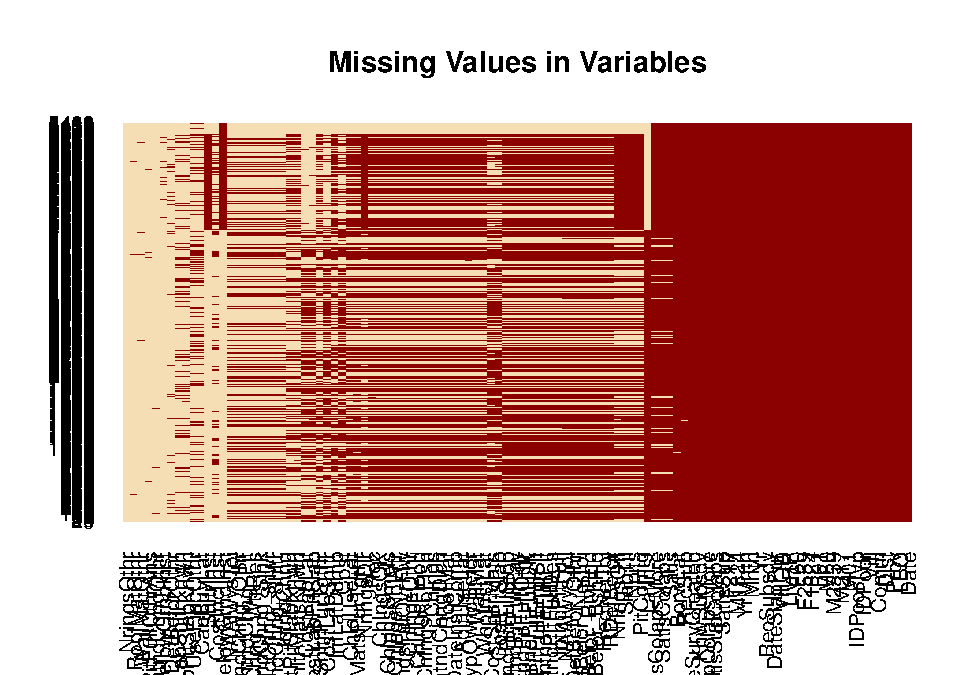
\includegraphics{describe_FSMintentions_regional_seasonal_iDE-Camb_surveysOct2017_files/figure-latex/summarize-1.pdf}

\begin{verbatim}
##   [1] "Date"                 "LBO"                  "Prov"                
##   [4] "Dist"                 "Comm"                 "Vill"                
##   [7] "IDPoor"               "IDPoorTyp"            "M01"                 
##  [10] "M1824"                "M217"                 "M2559"               
##  [13] "M60"                  "F01"                  "F1824"               
##  [16] "F217"                 "F2559"                "F60"                 
##  [19] "LivRP"                "VillOD"               "DateSlabPur"         
##  [22] "LatInst"              "BelowGrndInst"        "DateBelowGrndInst"   
##  [25] "ShltrInst"            "DateInstComp"         "RDefBefor"           
##  [28] "RDefBeforOthr"        "FreqNeiToi"           "WhoInstLat"          
##  [31] "KnwSubsdy"            "RecSubsdy"            "BorwLat"             
##  [34] "CanBuyLat"            "UseFincOthr"          "SlabTil"             
##  [37] "Npits"                "PitConfig"            "NringsDir"           
##  [40] "NringsOff"            "NringsOthr"           "WallMat"             
##  [43] "WallMatOthr"          "RoofMat"              "RoofMatOthr"         
##  [46] "MatsPurTgthr"         "Cost"                 "CostInclInst"        
##  [49] "CostPitSlab"          "CostPitSlabKnwn"      "CostShltrMats"       
##  [52] "CostShltrMatsKnwn"    "LabPitShltrPurTgthr"  "CostLabLat"          
##  [55] "CostLabPitSlab"       "CostLabPitSlabKnwn"   "CostLabShltr"        
##  [58] "CostLabShltrKnwn"     "LatTypOwndBefor"      "IntndChngDich"       
##  [61] "IntndChng"            "IntndChngOthr"        "AdltUseLat"          
##  [64] "ChldUseLat"           "InfLatDump"           "IntndPitFull"        
##  [67] "IntndPitFullOthrAns"  "Chlngs"               "Satis"               
##  [70] "Rec"                  "SatisSup"             "RecSup"              
##  [73] "DateSurvCreated"      "Yr"                   "Mnth"                
##  [76] "YrMnth"               "RDefBefor_BshFld"     "RDefBefor_RivPnd"    
##  [79] "RDefBefor_NeiToi"     "RDefBefor_Othr"       "RDefBefor_NAAlwysToi"
##  [82] "IntndChng_Shltr"      "IntndChng_Shwr"       "IntndChng_Sink"      
##  [85] "IntndChng_WtrRes"     "IntndChng_Pit"        "IntndChng_Othr"      
##  [88] "IntndChng_NAAlwysToi" "IntndPitFullDes"      "IntndPitFullPit"     
##  [91] "IntndPitFullEmpSlf"   "IntndPitFullDK"       "IntndPitFullOthr"    
##  [94] "IntndPitFullPay"      "IntndPitFullStop"     "ChlngsNoFlsh"        
##  [97] "ChlngsFlood"          "ChlngsOthr"           "ChlngsFulOvrFlw"     
## [100] "ChlngsNoWtr"          "ChlngsSmels"          "ChlngsOK"            
## [103] "SatisColaps"          "SatisSupColaps"       "SatisColapsMore"     
## [106] "SatisSupColapsMore"
\end{verbatim}

\includegraphics{describe_FSMintentions_regional_seasonal_iDE-Camb_surveysOct2017_files/figure-latex/MCA_setup-1.pdf}
\includegraphics{describe_FSMintentions_regional_seasonal_iDE-Camb_surveysOct2017_files/figure-latex/MCA_setup-2.pdf}
\includegraphics{describe_FSMintentions_regional_seasonal_iDE-Camb_surveysOct2017_files/figure-latex/MCA_setup-3.pdf}
\includegraphics{describe_FSMintentions_regional_seasonal_iDE-Camb_surveysOct2017_files/figure-latex/MCA_setup-4.pdf}
\includegraphics{describe_FSMintentions_regional_seasonal_iDE-Camb_surveysOct2017_files/figure-latex/MCA_setup-5.pdf}
\includegraphics{describe_FSMintentions_regional_seasonal_iDE-Camb_surveysOct2017_files/figure-latex/MCA_setup-6.pdf}
\includegraphics{describe_FSMintentions_regional_seasonal_iDE-Camb_surveysOct2017_files/figure-latex/MCA_setup-7.pdf}
\includegraphics{describe_FSMintentions_regional_seasonal_iDE-Camb_surveysOct2017_files/figure-latex/MCA_setup-8.pdf}
\includegraphics{describe_FSMintentions_regional_seasonal_iDE-Camb_surveysOct2017_files/figure-latex/MCA_setup-9.pdf}
\includegraphics{describe_FSMintentions_regional_seasonal_iDE-Camb_surveysOct2017_files/figure-latex/MCA_setup-10.pdf}

\begin{verbatim}
##                Prov      IDPoor      LivRP       VillOD    
##  Banteay Meanchey: 461   No :2818   No  :2918   Most: 288  
##  Kampong Thom    : 422   Yes: 903   Pond: 296   None: 207  
##  Kandal          :1002              Rivr: 507   Some:3226  
##  Oddar Meanchey  : 187                                     
##  Prey Veng       : 720                                     
##  Siem Reap       : 450                                     
##  Svay Rieng      : 479                                     
##                                                            
##                                                            
##                                                            
##                                                            
##                                                            
##        FreqNeiToi      WhoInstLat   KnwSubsdy   RecSubsdy    BorwLat    
##  Freq       : 443   Self/Fam:2365   No  :1757   DK   :   0   Yes : 943  
##  Nevr       :2872   Gov     :   2   Yes :1961   No   :3273   DK  :   0  
##  NA/AlwysToi:  78   Friend$ :  95   NA's:   3   Yfull:  33   No  :2744  
##  Some       : 328   Mason   : 883               Ypart: 415   NA's:  34  
##                     LBO     : 114                                       
##                     NGO     :  31                                       
##                     NA's    : 231                                       
##                                                                         
##                                                                         
##                                                                         
##                                                                         
##                                                                         
##  SlabTil                              WallMat    
##  No  :  84   Bamboo / Palm Leaves / Thatch: 374  
##  Yes :3404   Concrete / Brick             :1488  
##  NA's: 233   Galvanized steel             :1066  
##              No walls                     :  15  
##              Other                        :  68  
##              Plastic Sheet                : 338  
##              Wood                         : 140  
##              NA's                         : 232  
##                                                  
##                                                  
##                                                  
##                                                  
##                           RoofMat     AdltUseLat   ChldUseLat  
##  No roof                      : 349   Freq:3397   Freq  :2821  
##  Plastic Sheet                : 129   DK  :   1   NoChld:  20  
##  Galvanized steel             :2667   Rare:  22   DK/NA : 343  
##  Bamboo / Palm Leaves / Thatch: 278   Some:  68   Rare  :  89  
##  Concrete / Brick             :  18   NA's: 233   Some  : 163  
##  Other                        :  31               NA's  : 285  
##  Tiles                        :   5                            
##  Wood                         :  11                            
##  NA's                         : 233                            
##                                                                
##                                                                
##                                                                
##  InfLatDump      Yr       Mnth     RDefBefor_BshFld RDefBefor_RivPnd
##  Freq : 144   2014:   5   01:196   0: 823           0:3678          
##  NoInf:  89   2015: 620   02:198   1:2898           1:  43          
##  DK/NA:2314   2016:1195   03:203                                    
##  Rare : 586   2017:1901   04: 77                                    
##  Some : 115               05:267                                    
##  NA's : 473               06:242                                    
##                           07:176                                    
##                           08:529                                    
##                           09:361                                    
##                           10:411                                    
##                           11:598                                    
##                           12:463                                    
##  RDefBefor_NeiToi IntndPitFull  ChlngsNoFlsh ChlngsFlood ChlngsOthr 
##  0:3167           DK    : 613   0   :3251    0   :3452   0   :3404  
##  1: 554           EmpSlf: 782   1   : 234    1   :  33   1   :  81  
##                   Pit   : 883   NA's: 236    NA's: 236   NA's: 236  
##                   Othr  :  65                                       
##                   Pay   :1301                                       
##                   Stop  :  77                                       
##                                                                     
##                                                                     
##                                                                     
##                                                                     
##                                                                     
##                                                                     
##  ChlngsFulOvrFlw ChlngsNoWtr ChlngsSmels ChlngsOK    SatisColapsMore
##  0   :3463       0   :3458   0   :3401   0   : 426   1   : 457      
##  1   :  22       1   :  27   1   :  84   1   :3059   2   :2994      
##  NA's: 236       NA's: 236   NA's: 236   NA's: 236   DK  :  37      
##                                                      NA's: 233      
##                                                                     
##                                                                     
##                                                                     
##                                                                     
##                                                                     
##                                                                     
##                                                                     
##                                                                     
##  SatisSupColapsMore   Rec        RecSup          M01         
##  1   : 740          No  :1899   No  :2584   Min.   :0.00000  
##  2   :2895          Yes :1585   Yes :1128   1st Qu.:0.00000  
##  DK  :  84          NA's: 237   NA's:   9   Median :0.00000  
##  NA's:   2                                  Mean   :0.09191  
##                                             3rd Qu.:0.00000  
##                                             Max.   :2.00000  
##                                                              
##                                                              
##                                                              
##                                                              
##                                                              
##                                                              
##      M1824              M217            M2559            M60       
##  Min.   : 0.0000   Min.   :0.0000   Min.   :0.000   Min.   :0.000  
##  1st Qu.: 0.0000   1st Qu.:0.0000   1st Qu.:1.000   1st Qu.:0.000  
##  Median : 0.0000   Median :1.0000   Median :1.000   Median :0.000  
##  Mean   : 0.4465   Mean   :0.8159   Mean   :1.032   Mean   :0.161  
##  3rd Qu.: 1.0000   3rd Qu.:1.0000   3rd Qu.:1.000   3rd Qu.:0.000  
##  Max.   :18.0000   Max.   :9.0000   Max.   :6.000   Max.   :5.000  
##  NA's   :1                                                         
##                                                                    
##                                                                    
##                                                                    
##                                                                    
##                                                                    
##       F01             F1824             F217            F2559      
##  Min.   :0.0000   Min.   :0.0000   Min.   :0.0000   Min.   :0.000  
##  1st Qu.:0.0000   1st Qu.:0.0000   1st Qu.:0.0000   1st Qu.:1.000  
##  Median :0.0000   Median :0.0000   Median :1.0000   Median :1.000  
##  Mean   :0.0774   Mean   :0.4058   Mean   :0.8282   Mean   :1.121  
##  3rd Qu.:0.0000   3rd Qu.:1.0000   3rd Qu.:1.0000   3rd Qu.:1.000  
##  Max.   :8.0000   Max.   :8.0000   Max.   :9.0000   Max.   :6.000  
##                                    NA's   :1                       
##                                                                    
##                                                                    
##                                                                    
##                                                                    
##                                                                    
##       F60        
##  Min.   :0.0000  
##  1st Qu.:0.0000  
##  Median :0.0000  
##  Mean   :0.2435  
##  3rd Qu.:0.0000  
##  Max.   :2.0000  
##                  
##                  
##                  
##                  
##                  
## 
\end{verbatim}

\begin{verbatim}
##  Prov           IDPoor          LivWtr            VillOD    
##  BM:440   NotIDPoor:2652   LivWtr  : 757   MostVillOD: 220  
##  KT:385   IDPoor   : 785   NoLivWtr:2680   NoVillOD  : 197  
##  K :966                                    SomeVillOD:3020  
##  OM:152                                                     
##  PV:654                                                     
##  SR:400                                                     
##  SG:440                                                     
##                                                             
##                                                             
##                                                             
##                                                             
##                                                             
##       FreqNeiToi            WhoInstLat       KnwSubsdy        RecSubsdy   
##  FreqNeiToi: 413   Slf/FamInstLat:2349   KnwSubsdy:1637   NoSubsdy :3121  
##  NoNeiToi  :2648   FrndInstLat   :  95   DKSubsdy :1800   PrtSubsdy: 316  
##  AlwysToi  :  76   MasonInstLat  : 870                                    
##  SomeNeiToi: 300   LBOInstLat    : 110                                    
##                    NGOInstLat    :  13                                    
##                                                                           
##                                                                           
##                                                                           
##                                                                           
##                                                                           
##                                                                           
##                                                                           
##    BorwLat          SlabTil         WallMat          RoofMat    
##  Borw  : 858   NoSlabTil:  81   WoodWal : 508   NoRoof   : 346  
##  NoBorw:2579   SlabTil  :3356   MasnWal :1473   PlstcRoof: 129  
##                                 StelWal :1038   StelRoof :2626  
##                                 NoWal   :  15   WoodRoof : 284  
##                                 OthrWal :  68   MasnRoof :  16  
##                                 PlstcWal: 335   OthrRoof :  36  
##                                                                 
##                                                                 
##                                                                 
##                                                                 
##                                                                 
##                                                                 
##        AdltUseLat         ChldUseLat        InfLatDump      Yr      
##  AdltFreqLat:3347   ChldFreqLat:2777   InfFreqLat: 141   2015: 367  
##  AdltRarLat :  22   ChldDKLat  : 413   InfDKLat  :2608   2016:1183  
##  AdltSomLat :  68   ChldRarLat :  87   InfRarLat : 574   2017:1887  
##                     ChldSomLat : 160   InfSomLat : 114              
##                                                                     
##                                                                     
##                                                                     
##                                                                     
##                                                                     
##                                                                     
##                                                                     
##                                                                     
##  Mnth             RDefBefor_NeiToi IntndPitFull  ChlngsNoFlsh 
##  01:192   NoDefBeforNeiToi:2926    DK    : 571   FlshOK:3204  
##  02:198   DefBeforNeiToi  : 511    EmpSlf: 702   NoFlsh: 233  
##  03:203                            Pit   : 844                
##  04: 77                            Othr  :  64                
##  05:264                            Pay   :1190                
##  06:240                            Stop  :  66                
##  07:174                                                       
##  08:526                                                       
##  09:357                                                       
##  10:373                                                       
##  11:482                                                       
##  12:351                                                       
##   ChlngsFlood          ChlngsOthr      ChlngsFulOvrFlw ChlngsNoWtr 
##  NoFlood:3406   NoOthrChlngs:3358   NoFulOvrflw:3416   WtrOK:3411  
##  Flood  :  31   OthrChlngs  :  79   FulOvrflw  :  21   NoWtr:  26  
##                                                                    
##                                                                    
##                                                                    
##                                                                    
##                                                                    
##                                                                    
##                                                                    
##                                                                    
##                                                                    
##                                                                    
##  ChlngsSmels       ChlngsOK         Satis          SatisSup   
##  NoSmel:3356   Chlngs  : 418   UnsatLat: 452   UnsatSup: 661  
##  Smel  :  81   NoChlngs:3019   SatLat  :2948   SatSup  :2701  
##                                DKSatLat:  37   DKSatSup:  75  
##                                                               
##                                                               
##                                                               
##                                                               
##                                                               
##                                                               
##                                                               
##                                                               
##                                                               
##        Rec            RecSup          M01              M1824        
##  NoRecLat:1876   NoRecSup:2387   Min.   :0.00000   Min.   : 0.0000  
##  RecLat  :1561   RecSup  :1050   1st Qu.:0.00000   1st Qu.: 0.0000  
##                                  Median :0.00000   Median : 0.0000  
##                                  Mean   :0.09136   Mean   : 0.4454  
##                                  3rd Qu.:0.00000   3rd Qu.: 1.0000  
##                                  Max.   :2.00000   Max.   :18.0000  
##                                                                     
##                                                                     
##                                                                     
##                                                                     
##                                                                     
##                                                                     
##       M217            M2559            M60              F01         
##  Min.   :0.0000   Min.   :0.000   Min.   :0.0000   Min.   :0.00000  
##  1st Qu.:0.0000   1st Qu.:1.000   1st Qu.:0.0000   1st Qu.:0.00000  
##  Median :1.0000   Median :1.000   Median :0.0000   Median :0.00000  
##  Mean   :0.8118   Mean   :1.033   Mean   :0.1664   Mean   :0.07652  
##  3rd Qu.:1.0000   3rd Qu.:1.000   3rd Qu.:0.0000   3rd Qu.:0.00000  
##  Max.   :9.0000   Max.   :6.000   Max.   :5.0000   Max.   :8.00000  
##                                                                     
##                                                                     
##                                                                     
##                                                                     
##                                                                     
##                                                                     
##      F1824             F217            F2559            F60        
##  Min.   :0.0000   Min.   :0.0000   Min.   :0.000   Min.   :0.0000  
##  1st Qu.:0.0000   1st Qu.:0.0000   1st Qu.:1.000   1st Qu.:0.0000  
##  Median :0.0000   Median :1.0000   Median :1.000   Median :0.0000  
##  Mean   :0.4038   Mean   :0.8303   Mean   :1.128   Mean   :0.2459  
##  3rd Qu.:1.0000   3rd Qu.:1.0000   3rd Qu.:1.000   3rd Qu.:0.0000  
##  Max.   :8.0000   Max.   :9.0000   Max.   :6.000   Max.   :2.0000  
##                                                                    
##                                                                    
##                                                                    
##                                                                    
##                                                                    
##                                                                    
##       ODBefor    
##  NoODBefor: 754  
##  ODBefor  :2683  
##                  
##                  
##                  
##                  
##                  
##                  
##                  
##                  
##                  
## 
\end{verbatim}

\begin{verbatim}
##             Prov           IDPoor           LivWtr           VillOD 
##                0                0                0                0 
##       FreqNeiToi       WhoInstLat        KnwSubsdy        RecSubsdy 
##                0                0                0                0 
##          BorwLat          SlabTil          WallMat          RoofMat 
##                0                0                0                0 
##       AdltUseLat       ChldUseLat       InfLatDump               Yr 
##                0                0                0                0 
##             Mnth RDefBefor_NeiToi     IntndPitFull     ChlngsNoFlsh 
##                0                0                0                0 
##      ChlngsFlood       ChlngsOthr  ChlngsFulOvrFlw      ChlngsNoWtr 
##                0                0                0                0 
##      ChlngsSmels         ChlngsOK            Satis         SatisSup 
##                0                0                0                0 
##              Rec           RecSup              M01            M1824 
##                0                0                0                0 
##             M217            M2559              M60              F01 
##                0                0                0                0 
##            F1824             F217            F2559              F60 
##                0                0                0                0 
##          ODBefor 
##                0
\end{verbatim}

\includegraphics{describe_FSMintentions_regional_seasonal_iDE-Camb_surveysOct2017_files/figure-latex/MCA_setup-11.pdf}

\begin{verbatim}
##                name idx nobs    type exo user  mean   var nlev
## 1              Prov   1 3437  factor   0    0    NA    NA    7
## 2            IDPoor   2 3437  factor   0    0    NA    NA    2
## 3            LivWtr   3 3437  factor   0    0    NA    NA    2
## 4            VillOD   4 3437  factor   0    0    NA    NA    3
## 5        FreqNeiToi   5 3437  factor   0    0    NA    NA    4
## 6        WhoInstLat   6 3437  factor   0    0    NA    NA    5
## 7         KnwSubsdy   7 3437  factor   0    0    NA    NA    2
## 8         RecSubsdy   8 3437  factor   0    0    NA    NA    2
## 9           BorwLat   9 3437  factor   0    0    NA    NA    2
## 10          SlabTil  10 3437  factor   0    0    NA    NA    2
## 11          WallMat  11 3437  factor   0    0    NA    NA    6
## 12          RoofMat  12 3437  factor   0    0    NA    NA    6
## 13       AdltUseLat  13 3437  factor   0    0    NA    NA    3
## 14       ChldUseLat  14 3437  factor   0    0    NA    NA    4
## 15       InfLatDump  15 3437  factor   0    0    NA    NA    4
## 16               Yr  16 3437  factor   0    0    NA    NA    3
## 17             Mnth  17 3437  factor   0    0    NA    NA   12
## 18 RDefBefor_NeiToi  18 3437  factor   0    0    NA    NA    2
## 19     IntndPitFull  19 3437  factor   0    0    NA    NA    6
## 20     ChlngsNoFlsh  20 3437  factor   0    0    NA    NA    2
## 21      ChlngsFlood  21 3437  factor   0    0    NA    NA    2
## 22       ChlngsOthr  22 3437  factor   0    0    NA    NA    2
## 23  ChlngsFulOvrFlw  23 3437  factor   0    0    NA    NA    2
## 24      ChlngsNoWtr  24 3437  factor   0    0    NA    NA    2
## 25      ChlngsSmels  25 3437  factor   0    0    NA    NA    2
## 26         ChlngsOK  26 3437  factor   0    0    NA    NA    2
## 27            Satis  27 3437  factor   0    0    NA    NA    3
## 28         SatisSup  28 3437  factor   0    0    NA    NA    3
## 29              Rec  29 3437  factor   0    0    NA    NA    2
## 30           RecSup  30 3437  factor   0    0    NA    NA    2
## 31              M01  31 3437 numeric   0    0 0.091 0.089    0
## 32            M1824  32 3437 numeric   0    0 0.445 0.653    0
## 33             M217  33 3437 numeric   0    0 0.812 0.875    0
## 34            M2559  34 3437 numeric   0    0 1.033 0.458    0
## 35              M60  35 3437 numeric   0    0 0.166 0.146    0
## 36              F01  36 3437 numeric   0    0 0.077 0.095    0
## 37            F1824  37 3437 numeric   0    0 0.404 0.475    0
## 38             F217  38 3437 numeric   0    0 0.830 0.900    0
## 39            F2559  39 3437 numeric   0    0 1.128 0.386    0
## 40              F60  40 3437 numeric   0    0 0.246 0.199    0
## 41          ODBefor  41 3437  factor   0    0    NA    NA    2
##                                                             lnam
## 1                                            BM|KT|K|OM|PV|SR|SG
## 2                                               NotIDPoor|IDPoor
## 3                                                LivWtr|NoLivWtr
## 4                                 MostVillOD|NoVillOD|SomeVillOD
## 5                        FreqNeiToi|NoNeiToi|AlwysToi|SomeNeiToi
## 6  Slf/FamInstLat|FrndInstLat|MasonInstLat|LBOInstLat|NGOInstLat
## 7                                             KnwSubsdy|DKSubsdy
## 8                                             NoSubsdy|PrtSubsdy
## 9                                                    Borw|NoBorw
## 10                                             NoSlabTil|SlabTil
## 11                WoodWal|MasnWal|StelWal|NoWal|OthrWal|PlstcWal
## 12          NoRoof|PlstcRoof|StelRoof|WoodRoof|MasnRoof|OthrRoof
## 13                             AdltFreqLat|AdltRarLat|AdltSomLat
## 14                   ChldFreqLat|ChldDKLat|ChldRarLat|ChldSomLat
## 15                       InfFreqLat|InfDKLat|InfRarLat|InfSomLat
## 16                                                2015|2016|2017
## 17                           01|02|03|04|05|06|07|08|09|10|11|12
## 18                               NoDefBeforNeiToi|DefBeforNeiToi
## 19                                   DK|EmpSlf|Pit|Othr|Pay|Stop
## 20                                                 FlshOK|NoFlsh
## 21                                                 NoFlood|Flood
## 22                                       NoOthrChlngs|OthrChlngs
## 23                                         NoFulOvrflw|FulOvrflw
## 24                                                   WtrOK|NoWtr
## 25                                                   NoSmel|Smel
## 26                                               Chlngs|NoChlngs
## 27                                      UnsatLat|SatLat|DKSatLat
## 28                                      UnsatSup|SatSup|DKSatSup
## 29                                               NoRecLat|RecLat
## 30                                               NoRecSup|RecSup
## 31                                                              
## 32                                                              
## 33                                                              
## 34                                                              
## 35                                                              
## 36                                                              
## 37                                                              
## 38                                                              
## 39                                                              
## 40                                                              
## 41                                             NoODBefor|ODBefor
\end{verbatim}

\begin{Shaded}
\begin{Highlighting}[]
\KeywordTok{par}\NormalTok{(}\DataTypeTok{mfrow =} \KeywordTok{c}\NormalTok{(}\DecValTok{1}\NormalTok{, }\DecValTok{1}\NormalTok{))}
\KeywordTok{print}\NormalTok{(res.mca)}
\end{Highlighting}
\end{Shaded}

\begin{verbatim}
## **Results of the Multiple Correspondence Analysis (MCA)**
## The analysis was performed on 3437 individuals, described by 41 variables
## *The results are available in the following objects:
## 
##    name               
## 1  "$eig"             
## 2  "$var"             
## 3  "$var$coord"       
## 4  "$var$cos2"        
## 5  "$var$contrib"     
## 6  "$var$v.test"      
## 7  "$ind"             
## 8  "$ind$coord"       
## 9  "$ind$cos2"        
## 10 "$ind$contrib"     
## 11 "$quanti.sup"      
## 12 "$quanti.sup$coord"
## 13 "$quali.sup"       
## 14 "$quali.sup$coord" 
## 15 "$quali.sup$cos2"  
## 16 "$quali.sup$v.test"
## 17 "$call"            
## 18 "$call$marge.col"  
## 19 "$call$marge.li"   
##    description                                           
## 1  "eigenvalues"                                         
## 2  "results for the variables"                           
## 3  "coord. of the categories"                            
## 4  "cos2 for the categories"                             
## 5  "contributions of the categories"                     
## 6  "v-test for the categories"                           
## 7  "results for the individuals"                         
## 8  "coord. for the individuals"                          
## 9  "cos2 for the individuals"                            
## 10 "contributions of the individuals"                    
## 11 "results for the supplementary quantitative variables"
## 12 "coord. of the supplementary quantitative variables"  
## 13 "results for the supplementary categorical variables" 
## 14 "coord. for the supplementary categories"             
## 15 "cos2 for the supplementary categories"               
## 16 "v-test for the supplementary categories"             
## 17 "intermediate results"                                
## 18 "weights of columns"                                  
## 19 "weights of rows"
\end{verbatim}

\begin{Shaded}
\begin{Highlighting}[]
\KeywordTok{get_eigenvalue}\NormalTok{(res.mca)}
\end{Highlighting}
\end{Shaded}

\begin{verbatim}
##         eigenvalue variance.percent cumulative.variance.percent
## Dim.1  0.095099282       5.02411301                    5.024113
## Dim.2  0.086015833       4.54423269                    9.568346
## Dim.3  0.071923454       3.79972966                   13.368075
## Dim.4  0.068784294       3.63388723                   17.001963
## Dim.5  0.056595599       2.98995619                   19.991919
## Dim.6  0.054810324       2.89563974                   22.887559
## Dim.7  0.053854318       2.84513376                   25.732692
## Dim.8  0.051034490       2.69616176                   28.428854
## Dim.9  0.049579420       2.61929010                   31.048144
## Dim.10 0.047411947       2.50478213                   33.552926
## Dim.11 0.046394441       2.45102707                   36.003953
## Dim.12 0.044354061       2.34323343                   38.347187
## Dim.13 0.043292758       2.28716459                   40.634351
## Dim.14 0.042900221       2.26642675                   42.900778
## Dim.15 0.040519824       2.14066995                   45.041448
## Dim.16 0.040134419       2.12030893                   47.161757
## Dim.17 0.039361587       2.07948004                   49.241237
## Dim.18 0.038428707       2.03019582                   51.271433
## Dim.19 0.038214325       2.01887000                   53.290303
## Dim.20 0.037544405       1.98347802                   55.273781
## Dim.21 0.037097664       1.95987660                   57.233657
## Dim.22 0.036602357       1.93370942                   59.167367
## Dim.23 0.036454241       1.92588443                   61.093251
## Dim.24 0.035490894       1.87499064                   62.968242
## Dim.25 0.035380699       1.86916901                   64.837411
## Dim.26 0.034627493       1.82937701                   66.666788
## Dim.27 0.033470631       1.76825975                   68.435048
## Dim.28 0.033313788       1.75997370                   70.195021
## Dim.29 0.032910341       1.73865951                   71.933681
## Dim.30 0.032513003       1.71766807                   73.651349
## Dim.31 0.032262282       1.70442247                   75.355771
## Dim.32 0.031466206       1.66236558                   77.018137
## Dim.33 0.031181360       1.64731715                   78.665454
## Dim.34 0.030784046       1.62632696                   80.291781
## Dim.35 0.030587267       1.61593108                   81.907712
## Dim.36 0.029235096       1.54449563                   83.452208
## Dim.37 0.028623443       1.51218189                   84.964390
## Dim.38 0.027770623       1.46712726                   86.431517
## Dim.39 0.026321098       1.39054858                   87.822066
## Dim.40 0.024757767       1.30795752                   89.130023
## Dim.41 0.023983643       1.26706040                   90.397084
## Dim.42 0.023087391       1.21971124                   91.616795
## Dim.43 0.021674107       1.14504717                   92.761842
## Dim.44 0.020782383       1.09793724                   93.859779
## Dim.45 0.018985773       1.00302197                   94.862801
## Dim.46 0.017933536       0.94743211                   95.810233
## Dim.47 0.016481836       0.87073851                   96.680972
## Dim.48 0.015427169       0.81502025                   97.495992
## Dim.49 0.014014066       0.74036574                   98.236358
## Dim.50 0.012840028       0.67834110                   98.914699
## Dim.51 0.012093731       0.63891408                   99.553613
## Dim.52 0.006771343       0.35773131                   99.911344
## Dim.53 0.001678127       0.08865577                  100.000000
\end{verbatim}

\begin{Shaded}
\begin{Highlighting}[]
\KeywordTok{fviz_screeplot}\NormalTok{(res.mca, }\DataTypeTok{addlabels =} \OtherTok{TRUE}\NormalTok{, }\DataTypeTok{ylim =} \KeywordTok{c}\NormalTok{(}\DecValTok{0}\NormalTok{, }\DecValTok{50}\NormalTok{))}
\end{Highlighting}
\end{Shaded}

\includegraphics{describe_FSMintentions_regional_seasonal_iDE-Camb_surveysOct2017_files/figure-latex/MCA_results-1.pdf}

\begin{Shaded}
\begin{Highlighting}[]
\KeywordTok{fviz_mca_biplot}\NormalTok{(res.mca, }\DataTypeTok{repel =} \OtherTok{FALSE}\NormalTok{, }\DataTypeTok{ggtheme =} \KeywordTok{theme_minimal}\NormalTok{())}
\end{Highlighting}
\end{Shaded}

\includegraphics{describe_FSMintentions_regional_seasonal_iDE-Camb_surveysOct2017_files/figure-latex/MCA_results-2.pdf}

\begin{Shaded}
\begin{Highlighting}[]
\NormalTok{res.mca.vars =}\StringTok{ }\KeywordTok{get_mca_var}\NormalTok{(res.mca)}
\KeywordTok{fviz_mca_var}\NormalTok{(res.mca, }\DataTypeTok{choice =} \StringTok{"mca.cor"}\NormalTok{, }\DataTypeTok{repel =} \OtherTok{TRUE}\NormalTok{,      }\CommentTok{# Cor, vars & dims}
             \DataTypeTok{ggtheme =} \KeywordTok{theme_minimal}\NormalTok{())}
\end{Highlighting}
\end{Shaded}

\includegraphics{describe_FSMintentions_regional_seasonal_iDE-Camb_surveysOct2017_files/figure-latex/MCA_results-3.pdf}

\begin{Shaded}
\begin{Highlighting}[]
\KeywordTok{fviz_mca_var}\NormalTok{(res.mca, }\DataTypeTok{repel =} \OtherTok{TRUE}\NormalTok{, }\DataTypeTok{ggtheme =} \KeywordTok{theme_minimal}\NormalTok{())}
\end{Highlighting}
\end{Shaded}

\includegraphics{describe_FSMintentions_regional_seasonal_iDE-Camb_surveysOct2017_files/figure-latex/MCA_results-4.pdf}

\begin{Shaded}
\begin{Highlighting}[]
\KeywordTok{fviz_mca_var}\NormalTok{(res.mca, }\DataTypeTok{col.var =} \StringTok{"black"}\NormalTok{, }\DataTypeTok{shape.var =} \DecValTok{15}\NormalTok{, }\DataTypeTok{repel =} \OtherTok{TRUE}\NormalTok{)}
\end{Highlighting}
\end{Shaded}

\includegraphics{describe_FSMintentions_regional_seasonal_iDE-Camb_surveysOct2017_files/figure-latex/MCA_results-5.pdf}

\begin{Shaded}
\begin{Highlighting}[]
\KeywordTok{head}\NormalTok{(}\KeywordTok{round}\NormalTok{(res.mca.vars}\OperatorTok{$}\NormalTok{coord, }\DecValTok{2}\NormalTok{))}
\end{Highlighting}
\end{Shaded}

\begin{verbatim}
##            Dim 1 Dim 2 Dim 3 Dim 4 Dim 5
## NotIDPoor  -0.05  0.07 -0.02 -0.15  0.06
## IDPoor      0.17 -0.22  0.05  0.52 -0.22
## LivWtr      0.06  0.05 -0.15  0.15 -0.04
## NoLivWtr   -0.02 -0.02  0.04 -0.04  0.01
## MostVillOD  0.24 -0.57  0.28 -0.29  0.14
## NoVillOD    0.17  0.73  0.27  0.66 -0.08
\end{verbatim}

\begin{Shaded}
\begin{Highlighting}[]
\KeywordTok{head}\NormalTok{(}\KeywordTok{round}\NormalTok{(res.mca.vars}\OperatorTok{$}\NormalTok{coord, }\DecValTok{2}\NormalTok{))}
\end{Highlighting}
\end{Shaded}

\begin{verbatim}
##            Dim 1 Dim 2 Dim 3 Dim 4 Dim 5
## NotIDPoor  -0.05  0.07 -0.02 -0.15  0.06
## IDPoor      0.17 -0.22  0.05  0.52 -0.22
## LivWtr      0.06  0.05 -0.15  0.15 -0.04
## NoLivWtr   -0.02 -0.02  0.04 -0.04  0.01
## MostVillOD  0.24 -0.57  0.28 -0.29  0.14
## NoVillOD    0.17  0.73  0.27  0.66 -0.08
\end{verbatim}

\begin{Shaded}
\begin{Highlighting}[]
\KeywordTok{head}\NormalTok{(}\KeywordTok{round}\NormalTok{(res.mca.vars}\OperatorTok{$}\NormalTok{cos2, }\DecValTok{4}\NormalTok{))}
\end{Highlighting}
\end{Shaded}

\begin{verbatim}
##             Dim 1  Dim 2  Dim 3  Dim 4  Dim 5
## NotIDPoor  0.0088 0.0144 0.0009 0.0812 0.0138
## IDPoor     0.0088 0.0144 0.0009 0.0812 0.0138
## LivWtr     0.0009 0.0008 0.0063 0.0061 0.0005
## NoLivWtr   0.0009 0.0008 0.0063 0.0061 0.0005
## MostVillOD 0.0039 0.0224 0.0055 0.0056 0.0013
## NoVillOD   0.0017 0.0323 0.0045 0.0261 0.0004
\end{verbatim}

\begin{Shaded}
\begin{Highlighting}[]
\KeywordTok{corrplot}\NormalTok{(res.mca.vars}\OperatorTok{$}\NormalTok{cos2, }\DataTypeTok{is.corr =} \OtherTok{FALSE}\NormalTok{)}
\end{Highlighting}
\end{Shaded}

\includegraphics{describe_FSMintentions_regional_seasonal_iDE-Camb_surveysOct2017_files/figure-latex/MCA_results-6.pdf}

\begin{Shaded}
\begin{Highlighting}[]
\KeywordTok{fviz_mca_var}\NormalTok{(res.mca, }\DataTypeTok{col.var =} \StringTok{"cos2"}\NormalTok{,}
             \DataTypeTok{gradient.cols =} \KeywordTok{c}\NormalTok{(}\StringTok{"#00AFBB"}\NormalTok{, }\StringTok{"#E7B800"}\NormalTok{, }\StringTok{"#FC4E07"}\NormalTok{), }
             \DataTypeTok{repel =} \OtherTok{TRUE}\NormalTok{,}
             \DataTypeTok{ggtheme =} \KeywordTok{theme_minimal}\NormalTok{())}
\end{Highlighting}
\end{Shaded}

\includegraphics{describe_FSMintentions_regional_seasonal_iDE-Camb_surveysOct2017_files/figure-latex/MCA_results-7.pdf}

\begin{Shaded}
\begin{Highlighting}[]
\KeywordTok{fviz_mca_var}\NormalTok{(res.mca, }\DataTypeTok{alpha.var =} \StringTok{"cos2"}\NormalTok{,}
             \DataTypeTok{repel =} \OtherTok{TRUE}\NormalTok{,}
             \DataTypeTok{ggtheme =} \KeywordTok{theme_minimal}\NormalTok{())}
\end{Highlighting}
\end{Shaded}

\includegraphics{describe_FSMintentions_regional_seasonal_iDE-Camb_surveysOct2017_files/figure-latex/MCA_results-8.pdf}

\begin{Shaded}
\begin{Highlighting}[]
\KeywordTok{fviz_cos2}\NormalTok{(res.mca, }\DataTypeTok{choice =} \StringTok{"var"}\NormalTok{, }\DataTypeTok{axes =} \DecValTok{1}\OperatorTok{:}\DecValTok{2}\NormalTok{)}
\end{Highlighting}
\end{Shaded}

\includegraphics{describe_FSMintentions_regional_seasonal_iDE-Camb_surveysOct2017_files/figure-latex/MCA_results-9.pdf}

\begin{Shaded}
\begin{Highlighting}[]
\KeywordTok{head}\NormalTok{(}\KeywordTok{round}\NormalTok{(res.mca.vars}\OperatorTok{$}\NormalTok{contrib, }\DecValTok{3}\NormalTok{))}
\end{Highlighting}
\end{Shaded}

\begin{verbatim}
##            Dim 1 Dim 2 Dim 3 Dim 4 Dim 5
## NotIDPoor  0.075 0.137 0.010 0.962 0.198
## IDPoor     0.254 0.461 0.033 3.251 0.671
## LivWtr     0.027 0.027 0.244 0.248 0.023
## NoLivWtr   0.008 0.008 0.069 0.070 0.007
## MostVillOD 0.135 0.869 0.254 0.272 0.074
## NoVillOD   0.061 1.263 0.208 1.279 0.024
\end{verbatim}

\begin{Shaded}
\begin{Highlighting}[]
\KeywordTok{fviz_contrib}\NormalTok{(res.mca, }\DataTypeTok{choice =} \StringTok{"var"}\NormalTok{, }\DataTypeTok{axes =} \DecValTok{1}\NormalTok{, }\DataTypeTok{top =} \DecValTok{15}\NormalTok{)}
\end{Highlighting}
\end{Shaded}

\includegraphics{describe_FSMintentions_regional_seasonal_iDE-Camb_surveysOct2017_files/figure-latex/MCA_results-10.pdf}

\begin{Shaded}
\begin{Highlighting}[]
\KeywordTok{fviz_contrib}\NormalTok{(res.mca, }\DataTypeTok{choice =} \StringTok{"var"}\NormalTok{, }\DataTypeTok{axes =} \DecValTok{2}\NormalTok{, }\DataTypeTok{top =} \DecValTok{15}\NormalTok{)}
\end{Highlighting}
\end{Shaded}

\includegraphics{describe_FSMintentions_regional_seasonal_iDE-Camb_surveysOct2017_files/figure-latex/MCA_results-11.pdf}

\begin{Shaded}
\begin{Highlighting}[]
\KeywordTok{fviz_contrib}\NormalTok{(res.mca, }\DataTypeTok{choice =} \StringTok{"var"}\NormalTok{, }\DataTypeTok{axes =} \DecValTok{1}\OperatorTok{:}\DecValTok{2}\NormalTok{, }\DataTypeTok{top =} \DecValTok{15}\NormalTok{)}
\end{Highlighting}
\end{Shaded}

\includegraphics{describe_FSMintentions_regional_seasonal_iDE-Camb_surveysOct2017_files/figure-latex/MCA_results-12.pdf}

\begin{Shaded}
\begin{Highlighting}[]
\KeywordTok{fviz_mca_var}\NormalTok{(res.mca, }\DataTypeTok{col.var =} \StringTok{"contrib"}\NormalTok{,}
             \DataTypeTok{gradient.cols =} \KeywordTok{c}\NormalTok{(}\StringTok{"#00AFBB"}\NormalTok{, }\StringTok{"#E7B800"}\NormalTok{, }\StringTok{"#FC4E07"}\NormalTok{), }
             \DataTypeTok{repel =} \OtherTok{TRUE}\NormalTok{, }
             \DataTypeTok{ggtheme =} \KeywordTok{theme_minimal}\NormalTok{())}
\end{Highlighting}
\end{Shaded}

\includegraphics{describe_FSMintentions_regional_seasonal_iDE-Camb_surveysOct2017_files/figure-latex/MCA_results-13.pdf}

\begin{Shaded}
\begin{Highlighting}[]
\KeywordTok{fviz_mca_var}\NormalTok{(res.mca, }\DataTypeTok{alpha.var =} \StringTok{"contrib"}\NormalTok{,}
             \DataTypeTok{repel =} \OtherTok{TRUE}\NormalTok{,}
             \DataTypeTok{ggtheme =} \KeywordTok{theme_minimal}\NormalTok{())}
\end{Highlighting}
\end{Shaded}

\includegraphics{describe_FSMintentions_regional_seasonal_iDE-Camb_surveysOct2017_files/figure-latex/MCA_results-14.pdf}

\begin{Shaded}
\begin{Highlighting}[]
\NormalTok{res.mca.ind =}\StringTok{ }\KeywordTok{get_mca_ind}\NormalTok{(res.mca)}
\KeywordTok{print}\NormalTok{(res.mca.ind)}
\end{Highlighting}
\end{Shaded}

\begin{verbatim}
## Multiple Correspondence Analysis Results for individuals
##  ===================================================
##   Name       Description                       
## 1 "$coord"   "Coordinates for the individuals" 
## 2 "$cos2"    "Cos2 for the individuals"        
## 3 "$contrib" "contributions of the individuals"
\end{verbatim}

\begin{Shaded}
\begin{Highlighting}[]
\KeywordTok{head}\NormalTok{(res.mca.ind}\OperatorTok{$}\NormalTok{coord)}
\end{Highlighting}
\end{Shaded}

\begin{verbatim}
##            Dim 1       Dim 2       Dim 3       Dim 4        Dim 5
## 154 -0.240932934  0.27914189 -0.09847273  0.13755096 -0.004505266
## 155 -0.140426748 -0.25611141 -0.19948985  0.25789534 -0.151063757
## 156  0.501385740 -0.21275166 -0.41714123  0.12991465 -0.096105515
## 157  0.028059233 -0.17517766  0.18410213  0.19425809 -0.217321753
## 158 -0.131075218 -0.07847411  0.04550284 -0.10031911 -0.037179985
## 159  0.006733437 -0.14859122 -0.33604633  0.02250878 -0.096037171
\end{verbatim}

\begin{Shaded}
\begin{Highlighting}[]
\KeywordTok{head}\NormalTok{(res.mca.ind}\OperatorTok{$}\NormalTok{contrib)}
\end{Highlighting}
\end{Shaded}

\begin{verbatim}
##            Dim 1       Dim 2        Dim 3        Dim 4        Dim 5
## 154 1.775970e-02 0.026356764 0.0039226707 0.0080031039 1.043467e-05
## 155 6.033133e-03 0.022187068 0.0160987269 0.0281331379 1.173163e-02
## 156 7.691077e-02 0.015310451 0.0703908438 0.0071391658 4.748259e-03
## 157 2.408767e-04 0.010380052 0.0137109509 0.0159620780 2.427975e-02
## 158 5.256352e-03 0.002083027 0.0008375814 0.0042569496 7.106508e-04
## 159 1.387129e-05 0.007468414 0.0456823288 0.0002143064 4.741508e-03
\end{verbatim}

\begin{Shaded}
\begin{Highlighting}[]
\KeywordTok{head}\NormalTok{(res.mca.ind}\OperatorTok{$}\NormalTok{cos2)}
\end{Highlighting}
\end{Shaded}

\begin{verbatim}
##            Dim 1      Dim 2       Dim 3        Dim 4        Dim 5
## 154 5.539237e-02 0.07435456 0.009253149 0.0180544760 1.936862e-05
## 155 2.226336e-02 0.07405406 0.044929610 0.0750892973 2.576390e-02
## 156 8.971537e-02 0.01615358 0.062099650 0.0060233652 3.296245e-03
## 157 8.492946e-04 0.03310276 0.036561535 0.0407066180 5.094636e-02
## 158 4.632887e-02 0.01660593 0.005583257 0.0271380022 3.727597e-03
## 159 3.172318e-05 0.01544861 0.079013528 0.0003544925 6.453300e-03
\end{verbatim}

\begin{Shaded}
\begin{Highlighting}[]
\CommentTok{# fviz_mca_ind(res.mca, col.ind = "cos2", }
\CommentTok{#              gradient.cols = c("#00AFBB", "#E7B800", "#FC4E07"),}
\CommentTok{#              repel = TRUE,}
\CommentTok{#              ggtheme = theme_minimal())}
\KeywordTok{fviz_mca_ind}\NormalTok{(res.mca, }
             \DataTypeTok{label =} \StringTok{"none"}\NormalTok{, }\CommentTok{# hide individual labels}
             \DataTypeTok{habillage =}\NormalTok{ data.mca}\OperatorTok{$}\NormalTok{Prov, }\CommentTok{# color by groups }
             \CommentTok{# palette = c("#00AFBB", "#E7B800"),}
             \DataTypeTok{addEllipses =} \OtherTok{TRUE}\NormalTok{, }\DataTypeTok{ellipse.type =} \StringTok{"confidence"}\NormalTok{,}
             \DataTypeTok{ggtheme =} \KeywordTok{theme_minimal}\NormalTok{())}
\end{Highlighting}
\end{Shaded}

\includegraphics{describe_FSMintentions_regional_seasonal_iDE-Camb_surveysOct2017_files/figure-latex/MCA_results-15.pdf}

\hypertarget{introduction}{%
\section{Introduction}\label{introduction}}

Academic workflow, certainly in political science, is at a crossroads.
The \emph{American Journal of Political Science} (\emph{AJPS}) announced
a (my words)
\href{http://ajps.org/2015/03/26/the-ajps-replication-policy-innovations-and-revisions/}{``show
your work'' initiative} in which authors who are tentatively accepted
for publication at the journal must hand over the raw code and data that
produced the results shown in the manuscript. The editorial team at
\emph{AJPS} then reproduces the code from the manuscript. Pending
successful replication, the manuscript moves toward publication. The
\emph{AJPS} might be at the fore of this movement, and it could be the
most aggressive among political science journals, but other journals in
our field have signed the joint
\href{http://www.dartstatement.org/}{Data Access \& Research
Transparency} (DART) initiative. This, at a bare minimum, requires
uploading code from quantitatively-oriented published articles to
in-house directories hosted by the journal or to services like
\href{http://dataverse.org/}{Dataverse}.

There are workflow implications to the Lacour controversy as well.
Political science, for the foreseeable future, will struggle with the
extent of
\href{http://stanford.edu/~dbroock/broockman_kalla_aronow_lg_irregularities.pdf}{the
data fraud perpetrated by Michael Lacour} in an article co-authored with
Donald P. Green in \emph{Science}, the general scientific journal of
record in the United States. A failure to reproduce LaCour's results
with different samples uncovered a comprehensive effort by LaCour to
``fake'' data that provided results to what we felt or believed to be
true \href{http://chronicle.com/article/LAffaire-LaCour/230905/}{(i.e.
``truthiness'')}. However,
\href{http://kieranhealy.org/blog/archives/2015/05/20/fake-science-real-consequences/}{fake
data can have real consequences} for both the researcher and those who
want to learn from it and use it for various purposes. Even research
done honestly may suffer the same fate if researchers are not diligent
in their workflow.

These recent events underscore the DART push and cast a shadow over our
workflow. However, good workflow has always been an issue in our
discipline. Cloud storage services like
\href{http://www.dropbox.com}{Dropbox} are still relatively new among
political scientists. Without cloud storage, previous workflow left open
the possibility that work between a home computer and an office computer
was lost as a function of a corrupted thumb drive, an overheated power
supply, or, among other things, the wave of viruses that
\href{http://money.cnn.com/2003/11/05/technology/microsoftbounty/}{would
particularly affect Microsoft users every summer}. Social sciences,
\href{http://kieranhealy.org/blog/archives/2014/01/23/plain-text/}{unlike
engineering}, have traditionally relied on software like Microsoft Word
for manuscript preparation though any word processor reduces workflow to
a series of clicks and strokes on a keyboard. This is
\href{http://www.nytimes.com/2013/04/19/opinion/krugman-the-excel-depression.html}{a
terrible way to track changes} or maintain version control. The addition
of collaborators only compounds all the aforementioned issues. The
proverbial left hand may not know what the right hand is doing.

I think there is reason for optimism. We only struggle with it now
because we have tools like \href{http://rmarkdown.rstudio.com/}{R
Markdown} and \href{http://pandoc.org/}{Pandoc}, more generally, that
make significant strides in workflow. LaTeX resolved earlier issues of
corrupted binary files by reducing documents to raw markup that was
little more than raw text and revisions that could be easily kept as
\href{http://tex.stackexchange.com/questions/11177/how-to-write-hidden-notes-in-a-latex-file}{``commented''
text}. However, for all its benefits (including pretty PDFs),
\href{http://www-rohan.sdsu.edu/~aty/bibliog/latex/gripe.html}{LaTeX is
\emph{ugly} code} and does not provide means of seamlessly working with
the actual data analysis itself. R Markdown both eliminates markup and
allows the author and her collaborators to write and reproduce the
manuscript in one fell swoop.

\hypertarget{getting-started-with-yaml}{%
\section{Getting Started with YAML}\label{getting-started-with-yaml}}

The lion's share of a R Markdown document will be raw text, though the
front matter may be the most important part of the document. R Markdown
uses \href{http://www.yaml.org/}{YAML} for its metadata and the fields
differ from
\href{http://svmiller.com/blog/2015/02/moving-from-beamer-to-r-markdown/}{what
an author would use for a Beamer presentation}. I provide a sample YAML
metadata largely taken from this exact document and explain it below.

\begin{Shaded}
\begin{Highlighting}[]
\OperatorTok{---}
\NormalTok{output}\OperatorTok{:}\StringTok{ }
\StringTok{  }\NormalTok{pdf_document}\OperatorTok{:}
\StringTok{    }\NormalTok{citation_package}\OperatorTok{:}\StringTok{ }\NormalTok{natbib}
\NormalTok{    keep_tex}\OperatorTok{:}\StringTok{ }\NormalTok{true}
\NormalTok{    fig_caption}\OperatorTok{:}\StringTok{ }\NormalTok{true}
\NormalTok{    latex_engine}\OperatorTok{:}\StringTok{ }\NormalTok{pdflatex}
\NormalTok{    template}\OperatorTok{:}\StringTok{ }\ErrorTok{~/}\NormalTok{Dropbox}\OperatorTok{/}\NormalTok{miscelanea}\OperatorTok{/}\NormalTok{svm}\OperatorTok{-}\NormalTok{r}\OperatorTok{-}\NormalTok{markdown}\OperatorTok{-}\NormalTok{templates}\OperatorTok{/}\NormalTok{svm}\OperatorTok{-}\NormalTok{latex}\OperatorTok{-}\NormalTok{ms.tex}
\NormalTok{title}\OperatorTok{:}\StringTok{ "A Pandoc Markdown Article Starter and Template"}
\NormalTok{thanks}\OperatorTok{:}\StringTok{ "Replication files are available on the author's Github account..."}
\NormalTok{author}\OperatorTok{:}
\OperatorTok{-}\StringTok{ }\NormalTok{name}\OperatorTok{:}\StringTok{ }\NormalTok{Steven V. Miller}
\NormalTok{  affiliation}\OperatorTok{:}\StringTok{ }\NormalTok{Clemson University}
\OperatorTok{-}\StringTok{ }\NormalTok{name}\OperatorTok{:}\StringTok{ }\NormalTok{Mary Margaret Albright}
\NormalTok{  affiliation}\OperatorTok{:}\StringTok{ }\NormalTok{Pendelton State University}
\OperatorTok{-}\StringTok{ }\NormalTok{name}\OperatorTok{:}\StringTok{ }\NormalTok{Rembrandt Q. Einstein}
\NormalTok{  affiliation}\OperatorTok{:}\StringTok{ }\NormalTok{Springfield University}
\NormalTok{abstract}\OperatorTok{:}\StringTok{ "This document provides an introduction to R Markdown, argues for its..."}
\NormalTok{keywords}\OperatorTok{:}\StringTok{ "pandoc, r markdown, knitr"}
\NormalTok{date}\OperatorTok{:}\StringTok{ "`r format(Sys.time(), '%B %d, %Y')`"}
\NormalTok{geometry}\OperatorTok{:}\StringTok{ }\NormalTok{margin=1in}
\NormalTok{fontfamily}\OperatorTok{:}\StringTok{ }\NormalTok{mathpazo}
\NormalTok{fontsize}\OperatorTok{:}\StringTok{ }\NormalTok{11pt}
\CommentTok{# spacing: double}
\NormalTok{bibliography}\OperatorTok{:}\StringTok{ }\ErrorTok{~/}\NormalTok{Dropbox}\OperatorTok{/}\NormalTok{master.bib}
\NormalTok{biblio}\OperatorTok{-}\NormalTok{style}\OperatorTok{:}\StringTok{ }\NormalTok{apsr}
\OperatorTok{---}
\end{Highlighting}
\end{Shaded}

\texttt{output:} will tell R Markdown we want a PDF document rendered
with LaTeX. Since we are adding a fair bit of custom options to this
call, we specify \texttt{pdf\_document:} on the next line (with,
importantly, a two-space indent). We specify additional output-level
options underneath it, each are indented with four spaces.
\texttt{citation\_package:\ natbib} tells R Markdown to use
\texttt{natbib} to handle bibliographic citations.\footnote{R Markdown
  can use Pandoc's native bibliography management system or even
  \texttt{biblatex}, but I've found that it chokes with some of the more
  advanced stuff I've done with my .bib file over the years. For
  example, I've been diligent about special characters (e.g.~umlauts and
  acute accents) in author names in my .bib file, but Pandoc's native
  citation system will choke on these characters in a .bib file. I
  effectively need \texttt{natbib} for my own projects.} Thereafter, the
next line (\texttt{keep\_tex:\ true}) tells R Markdown to render a raw
\texttt{.tex} file along with the PDF document. This is useful for both
debugging and the publication stage, when the editorial team will ask
for the raw \texttt{.tex} so that they could render it and later provide
page proofs. The next line \texttt{fig\_caption:\ true} tells R Markdown
to make sure that whatever images are included in the document are
treated as figures in which our caption in brackets in a Markdown call
is treated as the caption in the figure. The next line
(\texttt{latex\_engine:\ pdflatex}) tells R Markdown to use pdflatex and
not some other option like \texttt{lualatex}. For my template, I'm
pretty sure this is mandatory.\footnote{The main reason I still use
  \texttt{pdflatex} (and most readers probably do as well) is because of
  LaTeX fonts.
  \href{http://www-rohan.sdsu.edu/~aty/bibliog/latex/gripe.html}{Unlike
  others}, I find standard LaTeX fonts to be appealing.}

The next line (\texttt{template:\ ...}) tells R Markdown to use my
custom LaTeX template.\footnote{Notice that the path is relative. The
  user can, if she wishes, install this in the default Pandoc directory.
  I don't think this is necessary. Just be mindful of wherever the
  template is placed. Importantly, \texttt{\textasciitilde{}} is used in
  R to find the home directory (not necessarily the working directory).
  It is equivalent to saying \texttt{/home/steve} in Linux, or
  \texttt{/Users/steve} on a Mac, in my case.} While I will own any
errors in the code, I confess to ``Frankensteining'' this template from
\href{https://github.com/jgm/pandoc-templates}{the default LaTeX
template} from Pandoc,
\href{https://github.com/kjhealy/pandoc-templates/tree/master/templates}{Kieran
Healy's LaTeX template}, and liberally using raw TeX from the
\href{https://www.acm.org/publications/article-templates/acm-latex-style-guide}{Association
for Computing Machinery's (ACM) LaTeX template}. I rather like that
template since it resembles standard manuscripts when they are published
in some of our more prominent journals. I will continue with a
description of the YAML metadata in the next paragraph, though invite
the curious reader to scroll to the end of the accompanying post to see
the PDF this template produces.

The next fields get to the heart of the document itself. \texttt{title:}
is, intuitively, the title of the manuscript. Do note that fields like
\texttt{title:} do not have to be in quotation marks, but must be in
quotation marks if the title of the document includes a colon. That
said, the only reason to use a colon in an article title is if it is
followed by a subtitle, hence the optional field (\texttt{subtitle:}).
Notice I ``comment out'' the subtitle in the above example with a pound
sign since this particular document does not have a subtitle. If
\texttt{thanks:} is included and has an accompanying entry, the ensuing
title of the document gets an asterisk and a footnote. This field is
typically used to advise readers that the document is a working paper or
is forthcoming in a journal.

The next field (\texttt{author:}) is a divergence from standard YAML,
but I think it is useful. I will also confess to pilfering this idea
from Kieran Healy's template. Typically, multiple authors for a given
document are separated by an \texttt{\textbackslash{}and} in this field.
However, standard LaTeX then creates a tabular field separating multiple
authors that is somewhat restrictive and not easy to override. As a
result, I use this setup (again, taken from Kieran Healy) to sidestep
the restrictive rendering of authors in the standard
\texttt{\textbackslash{}maketitle} tag. After \texttt{author:}, enter
\texttt{-\ name:} (no space before the dash) and fill in the field with
the first author. On the next line, enter two spaces, followed by
\texttt{affiliation:} and the institute or university affiliation of the
first author.

Do notice this can be repeated for however many co-authors there are to
a manuscript. The rendered PDF will enter each co-author in a new line
in a manner similar to journals like \emph{American Journal of Political
Science}, \emph{American Political Science Review}, or \emph{Journal of
Politics}.

The next two fields pertain to the frontmatter of a manuscript. They
should also be intuitive for the reader. \texttt{abstract} should
contain the abstract and \texttt{keywords} should contain some keywords
that describe the research project. Both fields are optional, though are
practically mandatory. Every manuscript requires an abstract and some
journals---especially those published by Sage---request them with
submitted manuscripts. My template also includes these keywords in the
PDF's metadata.

\texttt{date} comes standard with R Markdown and you can use it to enter
the date of the most recent compile. I typically include the date of the
last compile for a working paper in the \texttt{thanks:} field, so this
field currently does not do anything in my Markdown-LaTeX manuscript
template. I include it in my YAML as a legacy, basically.

The next items are optional and cosmetic. \texttt{geometry:} is a
standard option in LaTeX. I set the margins at one inch, and you
probably should too. \texttt{fontfamily:} is optional, but I use it to
specify the Palatino font. The default option is Computer Modern Roman.
\texttt{fontsize:} sets, intuitively, the font size. The default is
10-point, but I prefer 11-point. \texttt{spacing:} is an optional field.
If it is set as ``double'', the ensuing document is double-spaced.
``single'' is the only other valid entry for this field, though not
including the entry in the YAML metadata amounts to singlespacing the
document by default. Notice I have this ``commented out'' in the example
code.

The final two options pertain to the bibliography.
\texttt{bibliography:} specifies the location of the .bib file, so the
author could make citations in the manuscript. \texttt{biblio-style}
specifies the type of bibliography to use. You'll typically set this as
APSR. You could also specify the relative path of
\href{http://svmiller.com/miscellany/journal-of-peace-research-bst-file/}{my
\emph{Journal of Peace Research} .bst file} if you are submitting to
that journal.

\hypertarget{getting-started-with-markdown-syntax}{%
\section{Getting Started with Markdown
Syntax}\label{getting-started-with-markdown-syntax}}

There are a lot of cheatsheets and reference guides for Markdown (e.g.
\href{https://github.com/adam-p/markdown-here/wiki/Markdown-Cheatsheet}{Adam
Prichard},
\href{http://assemble.io/docs/Cheatsheet-Markdown.html}{Assemble},
\href{https://www.rstudio.com/wp-content/uploads/2015/02/rmarkdown-cheatsheet.pdf}{Rstudio},
\href{https://www.rstudio.com/wp-content/uploads/2015/03/rmarkdown-reference.pdf}{Rstudio
again},
\href{http://scottboms.com/downloads/documentation/markdown_cheatsheet.pdf}{Scott
Boms}, \href{https://daringfireball.net/projects/markdown/syntax}{Daring
Fireball}, among, I'm sure, several others). I encourage the reader to
look at those, though I will retread these references here with a
minimal working example below.

\begin{Shaded}
\begin{Highlighting}[]

\FunctionTok{# Introduction}

\NormalTok{**Lorem ipsum** dolor *sit amet*. }

\NormalTok{- }\FloatTok{Single asterisks italicize text *like this*. }
\FloatTok{- Double asterisks embolden text **like this**.}

\NormalTok{Start a new paragraph with a blank line separating paragraphs.}

\NormalTok{- }\FloatTok{This will start an unordered list environment, and this will be the first item.}
\FloatTok{- This will be a second item.}
\FloatTok{- A third item.}
\FloatTok{    - Four spaces and a dash create a sublist and this item in it.}
\FloatTok{- The fourth item.}
\FloatTok{    }
\FloatTok{1. This starts a numerical list.}
\FloatTok{2. This is no. 2 in the numerical list.}
\FloatTok{    }
\FloatTok{# This Starts A New Section}
\FloatTok{## This is a Subsection}
\FloatTok{### This is a Subsubsection}
\FloatTok{#### This starts a Paragraph Block.}

\NormalTok{>}\DataTypeTok{ This will create a block quote, if you want one.}

\NormalTok{Want a table? This will create one.}

\NormalTok{Table Header  | Second Header}
\NormalTok{------------- | -------------}
\NormalTok{Table Cell    | Cell 2}
\NormalTok{Cell 3        | Cell 4 }

\NormalTok{Note that the separators *do not* have to be aligned.}

\NormalTok{Want an image? This will do it.}

\AlertTok{![caption for my image](path/to/image.jpg)}

\BaseNTok{`fig_caption: yes`}\NormalTok{ will provide a caption. Put that in the YAML metadata.}

\NormalTok{Almost forgot about creating a footnote.}\OtherTok{[^1]}\NormalTok{ This will do it again.}\OtherTok{[^2]}

\OtherTok{[^1]}\NormalTok{: The first footnote}
\OtherTok{[^2]}\NormalTok{: The second footnote}

\NormalTok{Want to cite something? }

\NormalTok{- }\FloatTok{Find your biblatexkey in your bib file.}
\FloatTok{- Put an @ before it, like @smith1984, or whatever it is.}
\FloatTok{- @smith1984 creates an in-text citation (e.g. Smith (1984) says...)}
\FloatTok{- [@smith1984] creates a parenthetical citation (Smith, 1984)}

\NormalTok{That'll also automatically create a reference list at the end of the document.}

\OtherTok{[In-text link to Google](http://google.com)}\NormalTok{ as well.}
\end{Highlighting}
\end{Shaded}

That's honestly it. Markdown takes the chore of markup from your
manuscript (hence: ``Markdown'').

On that note, you could easily pass most LaTeX code through Markdown if
you're writing a LaTeX document. However, you don't need to do this
(unless you're using the math environment) and probably shouldn't anyway
if you intend to share your document in HTML as well.

\hypertarget{using-r-markdown-with-knitr}{%
\section{Using R Markdown with
Knitr}\label{using-r-markdown-with-knitr}}

Perhaps the greatest intrigue of R Markdown comes with the
\href{http://yihui.name/knitr/}{\texttt{knitr} package} provided by
\citet{xie2013ddrk}. In other words, the author can, if she chooses, do
the analysis in the Markdown document itself and compile/execute it in
R.

Take, for example, this simple exercise using the \texttt{voteincome}
data from the \texttt{Zelig} package. Suppose I want to explain the
decision to vote using data from this package. I load in the data, clean
the data, run the analyses, and present the results as a coefficient
plot.

Here's what this code looks like. All I did was create a code display,
which starts with three \emph{backticks} (i.e.~those ticks next to the
number 1 key on your keyboard) and ends with three backticks on another
line. On the first line of backticks (i.e.~to start the code display)
enter \texttt{\{r,\ eval=FALSE,\ tidy=TRUE\}}. The \texttt{eval=FALSE}
option just displays the R code (and does not run it),
\texttt{tidy=TRUE} wraps long code so it does not run off the page.

Within that code display, I enter my R code like this.

\begin{Shaded}
\begin{Highlighting}[]
\KeywordTok{suppressMessages}\NormalTok{(}\KeywordTok{library}\NormalTok{(Zelig))}
\KeywordTok{suppressMessages}\NormalTok{(}\KeywordTok{library}\NormalTok{(arm))}
\KeywordTok{suppressMessages}\NormalTok{(}\KeywordTok{library}\NormalTok{(coefplot))}

\KeywordTok{data}\NormalTok{(voteincome)}

\NormalTok{voteincome}\OperatorTok{$}\NormalTok{z.age <-}\StringTok{ }\NormalTok{arm}\OperatorTok{::}\KeywordTok{rescale}\NormalTok{(voteincome}\OperatorTok{$}\NormalTok{age)}
\NormalTok{voteincome}\OperatorTok{$}\NormalTok{z.education <-}\StringTok{ }\NormalTok{arm}\OperatorTok{::}\KeywordTok{rescale}\NormalTok{(voteincome}\OperatorTok{$}\NormalTok{education)}
\NormalTok{voteincome}\OperatorTok{$}\NormalTok{z.income <-}\StringTok{ }\NormalTok{arm}\OperatorTok{::}\KeywordTok{rescale}\NormalTok{(voteincome}\OperatorTok{$}\NormalTok{income)}

\NormalTok{M1 <-}\StringTok{ }\KeywordTok{glm}\NormalTok{(vote }\OperatorTok{~}\StringTok{ }\NormalTok{z.age }\OperatorTok{+}\StringTok{ }\NormalTok{female }\OperatorTok{+}\StringTok{ }\NormalTok{z.education }\OperatorTok{+}\StringTok{ }\NormalTok{z.income, }\DataTypeTok{data =}\NormalTok{ voteincome, }
    \DataTypeTok{family =}\NormalTok{ binomial)}

\KeywordTok{coefplot}\NormalTok{(M1)}
\end{Highlighting}
\end{Shaded}

The implications for workflow are faily substantial. Authors can rather
quickly display the code they used to run the analyses in the document
itself (likely in the appendix). As such, there's little guesswork for
reviewers and editors in understanding what the author did in the
analyses reported in the manuscript.

It doesn't end there. In fact, here's what happens when
\texttt{eval=FALSE} is omitted or changed to \texttt{eval=TRUE}. Now,
the code runs within R. Observe.

\begin{Shaded}
\begin{Highlighting}[]
\KeywordTok{suppressMessages}\NormalTok{(}\KeywordTok{library}\NormalTok{(Zelig))}
\end{Highlighting}
\end{Shaded}

\begin{verbatim}
## Warning: package 'Zelig' was built under R version 3.4.4
\end{verbatim}

\begin{Shaded}
\begin{Highlighting}[]
\KeywordTok{suppressMessages}\NormalTok{(}\KeywordTok{library}\NormalTok{(arm))}
\end{Highlighting}
\end{Shaded}

\begin{verbatim}
## Warning: package 'arm' was built under R version 3.4.4
\end{verbatim}

\begin{verbatim}
## Warning: package 'lme4' was built under R version 3.4.4
\end{verbatim}

\begin{Shaded}
\begin{Highlighting}[]
\KeywordTok{data}\NormalTok{(voteincome)}

\NormalTok{voteincome}\OperatorTok{$}\NormalTok{z.age <-}\StringTok{ }\NormalTok{arm}\OperatorTok{::}\KeywordTok{rescale}\NormalTok{(voteincome}\OperatorTok{$}\NormalTok{age)}
\NormalTok{voteincome}\OperatorTok{$}\NormalTok{z.education <-}\StringTok{ }\NormalTok{arm}\OperatorTok{::}\KeywordTok{rescale}\NormalTok{(voteincome}\OperatorTok{$}\NormalTok{education)}
\NormalTok{voteincome}\OperatorTok{$}\NormalTok{z.income <-}\StringTok{ }\NormalTok{arm}\OperatorTok{::}\KeywordTok{rescale}\NormalTok{(voteincome}\OperatorTok{$}\NormalTok{income)}

\NormalTok{M1 <-}\StringTok{ }\KeywordTok{glm}\NormalTok{(vote }\OperatorTok{~}\StringTok{ }\NormalTok{z.age }\OperatorTok{+}\StringTok{ }\NormalTok{female }\OperatorTok{+}\StringTok{ }\NormalTok{z.education }\OperatorTok{+}\StringTok{ }\NormalTok{z.income, }\DataTypeTok{data =}\NormalTok{ voteincome, }
    \DataTypeTok{family =}\NormalTok{ binomial)}

\NormalTok{arm}\OperatorTok{::}\KeywordTok{coefplot}\NormalTok{(M1)}
\end{Highlighting}
\end{Shaded}

\begin{figure}
\centering
\includegraphics{describe_FSMintentions_regional_seasonal_iDE-Camb_surveysOct2017_files/figure-latex/unnamed-chunk-3-1.pdf}
\caption{A Coefficient Plot}
\end{figure}

To get \texttt{knitr} to present the results of a table, add
\texttt{results="asis"} to the brackets to start the R code chunk. The
ensuing output will look like this (though the table may come on the
next page).

\begin{Shaded}
\begin{Highlighting}[]
\KeywordTok{suppressMessages}\NormalTok{(}\KeywordTok{library}\NormalTok{(Zelig))}
\KeywordTok{suppressMessages}\NormalTok{(}\KeywordTok{library}\NormalTok{(stargazer))}
\KeywordTok{suppressMessages}\NormalTok{(}\KeywordTok{library}\NormalTok{(arm))}

\KeywordTok{data}\NormalTok{(voteincome)}

\NormalTok{voteincome}\OperatorTok{$}\NormalTok{z.age <-}\StringTok{ }\NormalTok{arm}\OperatorTok{::}\KeywordTok{rescale}\NormalTok{(voteincome}\OperatorTok{$}\NormalTok{age)}
\NormalTok{voteincome}\OperatorTok{$}\NormalTok{z.education <-}\StringTok{ }\NormalTok{arm}\OperatorTok{::}\KeywordTok{rescale}\NormalTok{(voteincome}\OperatorTok{$}\NormalTok{education)}
\NormalTok{voteincome}\OperatorTok{$}\NormalTok{z.income <-}\StringTok{ }\NormalTok{arm}\OperatorTok{::}\KeywordTok{rescale}\NormalTok{(voteincome}\OperatorTok{$}\NormalTok{income)}


\NormalTok{M1 <-}\StringTok{ }\KeywordTok{glm}\NormalTok{(vote }\OperatorTok{~}\StringTok{ }\NormalTok{z.age }\OperatorTok{+}\StringTok{ }\NormalTok{female }\OperatorTok{+}\StringTok{ }\NormalTok{z.education }\OperatorTok{+}\StringTok{ }\NormalTok{z.income, }\DataTypeTok{data =}\NormalTok{ voteincome, }
    \DataTypeTok{family =}\NormalTok{ binomial)}

\KeywordTok{stargazer}\NormalTok{(M1, }\DataTypeTok{title =} \StringTok{"A Handsome Table"}\NormalTok{, }\DataTypeTok{header =} \OtherTok{FALSE}\NormalTok{)}
\end{Highlighting}
\end{Shaded}

\begin{table}[!htbp] \centering 
  \caption{A Handsome Table} 
  \label{} 
\begin{tabular}{@{\extracolsep{5pt}}lc} 
\\[-1.8ex]\hline 
\hline \\[-1.8ex] 
 & \multicolumn{1}{c}{\textit{Dependent variable:}} \\ 
\cline{2-2} 
\\[-1.8ex] & vote \\ 
\hline \\[-1.8ex] 
 z.age & 0.575$^{***}$ \\ 
  & (0.151) \\ 
  & \\ 
 female & 0.310$^{**}$ \\ 
  & (0.151) \\ 
  & \\ 
 z.education & 0.459$^{**}$ \\ 
  & (0.184) \\ 
  & \\ 
 z.income & 0.739$^{***}$ \\ 
  & (0.170) \\ 
  & \\ 
 Constant & 1.706$^{***}$ \\ 
  & (0.110) \\ 
  & \\ 
\hline \\[-1.8ex] 
Observations & 1,500 \\ 
Log Likelihood & $-$592.801 \\ 
Akaike Inf. Crit. & 1,195.602 \\ 
\hline 
\hline \\[-1.8ex] 
\textit{Note:}  & \multicolumn{1}{r}{$^{*}$p$<$0.1; $^{**}$p$<$0.05; $^{***}$p$<$0.01} \\ 
\end{tabular} 
\end{table}

Adding \texttt{echo="FALSE"} inside the brackets to start the R chunk
will omit the presentation of the R commands. It will just present the
table. This provides substantial opportunity for authors in doing their
analyses. Now, the analysis and presentation in the form of a polished
manuscript can be effectively simultaneous.\footnote{I'm not sure if I'm
  ready to commit to this myself since my workflow is still largely
  derived from
  \href{http://robjhyndman.com/hyndsight/workflow-in-r/}{Rob J.
  Hyndman's example}. However, \emph{knitr} has endless potential,
  especially when analyses can stored in cache, saved as chunks, or
  loaded in the preamble of a document to reference later in the
  manuscript.}




\newpage
\singlespacing 
\bibliography{\textasciitilde{}/Dropbox/master.bib}

\end{document}
